
%% bare_jrnl_compsoc.tex
%% V1.4b
%% 2015/08/26
%% by Michael Shell
%% See:
%% http://www.michaelshell.org/
%% for current contact information.
%%
%% This is a skeleton file demonstrating the use of IEEEtran.cls
%% (requires IEEEtran.cls version 1.8b or later) with an IEEE
%% Computer Society journal paper.
%%
%% Support sites:
%% http://www.michaelshell.org/tex/ieeetran/
%% http://www.ctan.org/pkg/ieeetran
%% and
%% http://www.ieee.org/



% *** Authors should verify (and, if needed, correct) their LaTeX system  ***
% *** with the testflow diagnostic prior to trusting their LaTeX platform ***
% *** with production work. The IEEE's font choices and paper sizes can   ***
% *** trigger bugs that do not appear when using other class files.       ***                          ***
% The testflow support page is at:
% http://www.michaelshell.org/tex/testflow/


\documentclass[10pt,journal,compsoc]{IEEEtran}


%
% If IEEEtran.cls has not been installed into the LaTeX system files,
% manually specify the path to it like:
% \documentclass[10pt,journal,compsoc]{../sty/IEEEtran}





% Some very useful LaTeX packages include:
% (uncomment the ones you want to load)


% *** MISC UTILITY PACKAGES ***
%
%\usepackage{ifpdf}
% Heiko Oberdiek's ifpdf.sty is very useful if you need conditional
% compilation based on whether the output is pdf or dvi.
% usage:
% \ifpdf
%   % pdf code
% \else
%   % dvi code
% \fi
% The latest version of ifpdf.sty can be obtained from:
% http://www.ctan.org/pkg/ifpdf
% Also, note that IEEEtran.cls V1.7 and later provides a builtin
% \ifCLASSINFOpdf conditional that works the same way.
% When switching from latex to pdflatex and vice-versa, the compiler may
% have to be run twice to clear warning/error messages.

\usepackage{color}

\usepackage{graphicx}
\usepackage{caption}
\usepackage{subcaption}
\usepackage{wrapfig}
\usepackage{hyperref}

%for tables
\usepackage{booktabs}
\usepackage{makecell}

%for algorithm
\usepackage{algorithm}
\usepackage[noend]{algpseudocode}
\usepackage{varwidth}

\usepackage{etex}

%% editing comment
\newcommand{\cmt}[1]{{\footnotesize\textcolor{red}{#1}}}
\newcommand{\note}[1]{\cmt{Note: #1}}
\newcommand{\todo}[1]{\cmt{TO-DO: #1}}
\newcommand{\sergey}[1]{\cmt{Sergey: #1}}
\newcommand{\chelsea}[1]{\cmt{Chelsea: #1}}
\newcommand{\pieter}[1]{\cmt{Pieter: #1}}

%% ignore text
\long\def\ignorethis#1{}

%% abbreviations
\newcommand{\etal}{{et~al.}\ }
\newcommand{\eg}{e.g.\ }
\newcommand{\ie}{i.e.\ }
\newcommand{\nth}{\text{th}}
\newcommand{\pr}{^\prime}
\newcommand{\tr}{^\mathrm{T}}
\newcommand{\inv}{^{-1}}
\newcommand{\pinv}{^{\dagger}}
\newcommand{\real}{\mathbb{R}}
\newcommand{\gauss}{\mathcal{N}}
\newcommand{\norm}[1]{\left|#1\right|}
\newcommand{\trace}{\text{tr}}

%% defines autoref commands
\def\sectionautorefname{Section}
\let\subsectionautorefname\sectionautorefname
\let\subsubsectionautorefname\sectionautorefname
\providecommand\algorithmname{Algorithm}
\def\equationautorefname~#1\null{Equation~(#1)\null}
\def\appendixautorefname{Appendix}

%% reference shortcuts
\newcommand{\figtodo}[1]{\framebox[0.8\columnwidth]{\rule{0pt}{1in}#1}}
\newcommand{\figref}[1]{\autoref{#1}}
%\renewcommand{\eqref}[1]{\autoref{#1}}
\newcommand{\secref}[1]{\autoref{#1}}

%% citation shortcuts
\newcommand{\atari}{acvpa-oglls-15}
\newcommand{\nyu}{vpbmse-mcl-16}

\newcommand{\model}{\mathcal{M}}
\newcommand{\action}{\mathbf{a}}
\newcommand{\state}{\mathbf{x}}
\newcommand{\image}{I_t}
\newcommand{\flow}{\hat{F}}
\newcommand{\pixel}{d} % the designated pixel
\newcommand{\pixelstate}{s} % the state of the desginated pixel
\newcommand{\goal}{g}




\usepackage{xcolor}  % for colored text
\providecommand\todo[1]{\textcolor{Red}{#1}}
\providecommand\edit[1]{\textcolor{blue}{#1}}



% *** CITATION PACKAGES ***
%
\ifCLASSOPTIONcompsoc
  % IEEE Computer Society needs nocompress option
  % requires cite.sty v4.0 or later (November 2003)
  \usepackage[nocompress]{cite}
\else
  % normal IEEE
  \usepackage{cite}
\fi
% cite.sty was written by Donald Arseneau
% V1.6 and later of IEEEtran pre-defines the format of the cite.sty package
% \cite{} output to follow that of the IEEE. Loading the cite package will
% result in citation numbers being automatically sorted and properly
% "compressed/ranged". e.g., [1], [9], [2], [7], [5], [6] without using
% cite.sty will become [1], [2], [5]--[7], [9] using cite.sty. cite.sty's
% \cite will automatically add leading space, if needed. Use cite.sty's
% noadjust option (cite.sty V3.8 and later) if you want to turn this off
% such as if a citation ever needs to be enclosed in parenthesis.
% cite.sty is already installed on most LaTeX systems. Be sure and use
% version 5.0 (2009-03-20) and later if using hyperref.sty.
% The latest version can be obtained at:
% http://www.ctan.org/pkg/cite
% The documentation is contained in the cite.sty file itself.
%
% Note that some packages require special options to format as the Computer
% Society requires. In particular, Computer Society  papers do not use
% compressed citation ranges as is done in typical IEEE papers
% (e.g., [1]-[4]). Instead, they list every citation separately in order
% (e.g., [1], [2], [3], [4]). To get the latter we need to load the cite
% package with the nocompress option which is supported by cite.sty v4.0
% and later. Note also the use of a CLASSOPTION conditional provided by
% IEEEtran.cls V1.7 and later.





% *** GRAPHICS RELATED PACKAGES ***
%
\ifCLASSINFOpdf
  % \usepackage[pdftex]{graphicx}
  % declare the path(s) where your graphic files are
  % \graphicspath{{../pdf/}{../jpeg/}}
  % and their extensions so you won't have to specify these with
  % every instance of \includegraphics
  % \DeclareGraphicsExtensions{.pdf,.jpeg,.png}
\else
  % or other class option (dvipsone, dvipdf, if not using dvips). graphicx
  % will default to the driver specified in the system graphics.cfg if no
  % driver is specified.
  % \usepackage[dvips]{graphicx}
  % declare the path(s) where your graphic files are
  % \graphicspath{{../eps/}}
  % and their extensions so you won't have to specify these with
  % every instance of \includegraphics
  % \DeclareGraphicsExtensions{.eps}
\fi
% graphicx was written by David Carlisle and Sebastian Rahtz. It is
% required if you want graphics, photos, etc. graphicx.sty is already
% installed on most LaTeX systems. The latest version and documentation
% can be obtained at: 
% http://www.ctan.org/pkg/graphicx
% Another good source of documentation is "Using Imported Graphics in
% LaTeX2e" by Keith Reckdahl which can be found at:
% http://www.ctan.org/pkg/epslatex
%
% latex, and pdflatex in dvi mode, support graphics in encapsulated
% postscript (.eps) format. pdflatex in pdf mode supports graphics
% in .pdf, .jpeg, .png and .mps (metapost) formats. Users should ensure
% that all non-photo figures use a vector format (.eps, .pdf, .mps) and
% not a bitmapped formats (.jpeg, .png). The IEEE frowns on bitmapped formats
% which can result in "jaggedy"/blurry rendering of lines and letters as
% well as large increases in file sizes.
%
% You can find documentation about the pdfTeX application at:
% http://www.tug.org/applications/pdftex






% *** MATH PACKAGES ***
%
%\usepackage{amsmath}
% A popular package from the American Mathematical Society that provides
% many useful and powerful commands for dealing with mathematics.
%
% Note that the amsmath package sets \interdisplaylinepenalty to 10000
% thus preventing page breaks from occurring within multiline equations. Use:
%\interdisplaylinepenalty=2500
% after loading amsmath to restore such page breaks as IEEEtran.cls normally
% does. amsmath.sty is already installed on most LaTeX systems. The latest
% version and documentation can be obtained at:
% http://www.ctan.org/pkg/amsmath

\usepackage{amsmath}
\usepackage{amsfonts}
\usepackage{mathtools}



% *** SPECIALIZED LIST PACKAGES ***
%
%\usepackage{algorithmic}
% algorithmic.sty was written by Peter Williams and Rogerio Brito.
% This package provides an algorithmic environment fo describing algorithms.
% You can use the algorithmic environment in-text or within a figure
% environment to provide for a floating algorithm. Do NOT use the algorithm
% floating environment provided by algorithm.sty (by the same authors) or
% algorithm2e.sty (by Christophe Fiorio) as the IEEE does not use dedicated
% algorithm float types and packages that provide these will not provide
% correct IEEE style captions. The latest version and documentation of
% algorithmic.sty can be obtained at:
% http://www.ctan.org/pkg/algorithms
% Also of interest may be the (relatively newer and more customizable)
% algorithmicx.sty package by Szasz Janos:
% http://www.ctan.org/pkg/algorithmicx




% *** ALIGNMENT PACKAGES ***
%
%\usepackage{array}
% Frank Mittelbach's and David Carlisle's array.sty patches and improves
% the standard LaTeX2e array and tabular environments to provide better
% appearance and additional user controls. As the default LaTeX2e table
% generation code is lacking to the point of almost being broken with
% respect to the quality of the end results, all users are strongly
% advised to use an enhanced (at the very least that provided by array.sty)
% set of table tools. array.sty is already installed on most systems. The
% latest version and documentation can be obtained at:
% http://www.ctan.org/pkg/array


% IEEEtran contains the IEEEeqnarray family of commands that can be used to
% generate multiline equations as well as matrices, tables, etc., of high
% quality.

%for tables
\usepackage{makecell}




% *** SUBFIGURE PACKAGES ***
%\ifCLASSOPTIONcompsoc
%  \usepackage[caption=false,font=footnotesize,labelfont=sf,textfont=sf]{subfig}
%\else
%  \usepackage[caption=false,font=footnotesize]{subfig}
%\fi
% subfig.sty, written by Steven Douglas Cochran, is the modern replacement
% for subfigure.sty, the latter of which is no longer maintained and is
% incompatible with some LaTeX packages including fixltx2e. However,
% subfig.sty requires and automatically loads Axel Sommerfeldt's caption.sty
% which will override IEEEtran.cls' handling of captions and this will result
% in non-IEEE style figure/table captions. To prevent this problem, be sure
% and invoke subfig.sty's "caption=false" package option (available since
% subfig.sty version 1.3, 2005/06/28) as this is will preserve IEEEtran.cls
% handling of captions.
% Note that the Computer Society format requires a sans serif font rather
% than the serif font used in traditional IEEE formatting and thus the need
% to invoke different subfig.sty package options depending on whether
% compsoc mode has been enabled.
%
% The latest version and documentation of subfig.sty can be obtained at:
% http://www.ctan.org/pkg/subfig




% *** FLOAT PACKAGES ***
%
%\usepackage{fixltx2e}
% fixltx2e, the successor to the earlier fix2col.sty, was written by
% Frank Mittelbach and David Carlisle. This package corrects a few problems
% in the LaTeX2e kernel, the most notable of which is that in current
% LaTeX2e releases, the ordering of single and double column floats is not
% guaranteed to be preserved. Thus, an unpatched LaTeX2e can allow a
% single column figure to be placed prior to an earlier double column
% figure.
% Be aware that LaTeX2e kernels dated 2015 and later have fixltx2e.sty's
% corrections already built into the system in which case a warning will
% be issued if an attempt is made to load fixltx2e.sty as it is no longer
% needed.
% The latest version and documentation can be found at:
% http://www.ctan.org/pkg/fixltx2e


%\usepackage{stfloats}
% stfloats.sty was written by Sigitas Tolusis. This package gives LaTeX2e
% the ability to do double column floats at the bottom of the page as well
% as the top. (e.g., "\begin{figure*}[!b]" is not normally possible in
% LaTeX2e). It also provides a command:
%\fnbelowfloat
% to enable the placement of footnotes below bottom floats (the standard
% LaTeX2e kernel puts them above bottom floats). This is an invasive package
% which rewrites many portions of the LaTeX2e float routines. It may not work
% with other packages that modify the LaTeX2e float routines. The latest
% version and documentation can be obtained at:
% http://www.ctan.org/pkg/stfloats
% Do not use the stfloats baselinefloat ability as the IEEE does not allow
% \baselineskip to stretch. Authors submitting work to the IEEE should note
% that the IEEE rarely uses double column equations and that authors should try
% to avoid such use. Do not be tempted to use the cuted.sty or midfloat.sty
% packages (also by Sigitas Tolusis) as the IEEE does not format its papers in
% such ways.
% Do not attempt to use stfloats with fixltx2e as they are incompatible.
% Instead, use Morten Hogholm'a dblfloatfix which combines the features
% of both fixltx2e and stfloats:
%
% \usepackage{dblfloatfix}
% The latest version can be found at:
% http://www.ctan.org/pkg/dblfloatfix



%\ifCLASSOPTIONcaptionsoff
%  \usepackage[nomarkers]{endfloat}
% \let\MYoriglatexcaption\caption
% \renewcommand{\caption}[2][\relax]{\MYoriglatexcaption[#2]{#2}}
%\fi
% endfloat.sty was written by James Darrell McCauley, Jeff Goldberg and 
% Axel Sommerfeldt. This package may be useful when used in conjunction with 
% IEEEtran.cls'  captionsoff option. Some IEEE journals/societies require that
% submissions have lists of figures/tables at the end of the paper and that
% figures/tables without any captions are placed on a page by themselves at
% the end of the document. If needed, the draftcls IEEEtran class option or
% \CLASSINPUTbaselinestretch interface can be used to increase the line
% spacing as well. Be sure and use the nomarkers option of endfloat to
% prevent endfloat from "marking" where the figures would have been placed
% in the text. The two hack lines of code above are a slight modification of
% that suggested by in the endfloat docs (section 8.4.1) to ensure that
% the full captions always appear in the list of figures/tables - even if
% the user used the short optional argument of \caption[]{}.
% IEEE papers do not typically make use of \caption[]'s optional argument,
% so this should not be an issue. A similar trick can be used to disable
% captions of packages such as subfig.sty that lack options to turn off
% the subcaptions:
% For subfig.sty:
% \let\MYorigsubfloat\subfloat
% \renewcommand{\subfloat}[2][\relax]{\MYorigsubfloat[]{#2}}
% However, the above trick will not work if both optional arguments of
% the \subfloat command are used. Furthermore, there needs to be a
% description of each subfigure *somewhere* and endfloat does not add
% subfigure captions to its list of figures. Thus, the best approach is to
% avoid the use of subfigure captions (many IEEE journals avoid them anyway)
% and instead reference/explain all the subfigures within the main caption.
% The latest version of endfloat.sty and its documentation can obtained at:
% http://www.ctan.org/pkg/endfloat
%
% The IEEEtran \ifCLASSOPTIONcaptionsoff conditional can also be used
% later in the document, say, to conditionally put the References on a 
% page by themselves.




% *** PDF, URL AND HYPERLINK PACKAGES ***
%
%\usepackage{url}
% url.sty was written by Donald Arseneau. It provides better support for
% handling and breaking URLs. url.sty is already installed on most LaTeX
% systems. The latest version and documentation can be obtained at:
% http://www.ctan.org/pkg/url
% Basically, \url{my_url_here}.

\usepackage{babel}
\usepackage{cuted}



% *** Do not adjust lengths that control margins, column widths, etc. ***
% *** Do not use packages that alter fonts (such as pslatex).         ***
% There should be no need to do such things with IEEEtran.cls V1.6 and later.
% (Unless specifically asked to do so by the journal or conference you plan
% to submit to, of course. )


% correct bad hyphenation here
\hyphenation{op-tical net-works semi-conduc-tor}


\begin{document}
%
% paper title
% Titles are generally capitalized except for words such as a, an, and, as,
% at, but, by, for, in, nor, of, on, or, the, to and up, which are usually
% not capitalized unless they are the first or last word of the title.
% Linebreaks \\ can be used within to get better formatting as desired.
% Do not put math or special symbols in the title.
%\title{Deep Reinforcement Learning with Observation Models}
\title{Visual Foresight: Model-Based Deep Reinforcement Learning for Vision-Based Robotic Control}
%14: I think the current title is a bit too aggressive -- kind of makes it seem like all the other RL is not "real." We should make sure to hit a few key words: we need to make sure the title communicates that this is based on images, that there is robotic manipulation going on, and that it is based on prediction or something like that. We should also pick a name for the method. I don't particularly like "Visual MPC" (it sounds a bit antiquated, like visual servoing), but if we go with that, we can call it
%Visual MPC: Model-Based Deep Reinforcement Learning for Vision-Based Robotic Control
% we can also go with "foresight" and call it
%Visual Foresight: Deep Reinforcement Learning via Prediction for Vision-Based Robotic Control
%% Real-World Deep Reinforcement Learning with Sensory Prediction Models
%% TITLE IDEAS HERE (separate from method names)
% Learning Observation Models for Real-World Planning and Control
% Deep Reinforcement Learning from Images with Observation Models
% Observation Models for Scalable, Real-World Reinforcement Learning
% Observation Models for Scalable Deep Reinforcement Learning
%
% Robotic Manipluation using Video Prediction Models
% Deep Model-Based Reinforcement Learning for Real-World Visual Control
% Deep Visual Predictive Models for Control
% Predictive Models for Visual Planning
% Deep Predictive Models for Visual Planning
% Learning Visual Foresight for Robotic Manipulation
% Observation Models for Self-Supervised Planning and Control
% Learning Observation Models for Real-World Planning and Control
% Learning Observation Models for Planning and Control
% Observation Models for Real-World Reinforcement Learning
%
% Sensory Prediction Models for Real-World Reinforcement Learning
% Sensory Prediction Models for Real-World Deep Reinforcement Learning

\author{Frederik Ebert*, Chelsea Finn*, Sudeep Dasari, Annie Xie, Alex Lee, Sergey Levine
%Frederik Ebert, Chelsea Finn, Alex Lee, Annie Xie, Sudeep Dasari, Sergey Levine
        
\IEEEcompsocitemizethanks{
\IEEEcompsocthanksitem  The first two authors contributed equally.}% <-this % stops an unwanted space
\thanks{Manuscript received 11/22/2018}}

% note the % following the last \IEEEmembership and also \thanks - 
% these prevent an unwanted space from occurring between the last author name
% and the end of the author line. i.e., if you had this:
% 
% \author{....lastname \thanks{...} \thanks{...} }
%                     ^------------^------------^----Do not want these spaces!
%
% a space would be appended to the last name and could cause every name on that
% line to be shifted left slightly. This is one of those "LaTeX things". For
% instance, "\textbf{A} \textbf{B}" will typeset as "A B" not "AB". To get
% "AB" then you have to do: "\textbf{A}\textbf{B}"
% \thanks is no different in this regard, so shield the last } of each \thanks
% that ends a line with a % and do not let a space in before the next \thanks.
% Spaces after \IEEEmembership other than the last one are OK (and needed) as
% you are supposed to have spaces between the names. For what it is worth,
% this is a minor point as most people would not even notice if the said evil
% space somehow managed to creep in.



% The paper headers
\markboth{Journal of \LaTeX\ Class Files,~Vol.~14, No.~8, August~2015}%
{Shell \MakeLowercase{\textit{et al.}}: Bare Demo of IEEEtran.cls for Computer Society Journals}
% The only time the second header will appear is for the odd numbered pages
% after the title page when using the twoside option.
% 
% *** Note that you probably will NOT want to include the author's ***
% *** name in the headers of peer review papers.                   ***
% You can use \ifCLASSOPTIONpeerreview for conditional compilation here if
% you desire.



% The publisher's ID mark at the bottom of the page is less important with
% Computer Society journal papers as those publications place the marks
% outside of the main text columns and, therefore, unlike regular IEEE
% journals, the available text space is not reduced by their presence.
% If you want to put a publisher's ID mark on the page you can do it like
% this:
%\IEEEpubid{0000--0000/00\$00.00~\copyright~2015 IEEE}
% or like this to get the Computer Society new two part style.
%\IEEEpubid{\makebox[\columnwidth]{\hfill 0000--0000/00/\$00.00~\copyright~2015 IEEE}%
%\hspace{\columnsep}\makebox[\columnwidth]{Published by the IEEE Computer Society\hfill}}
% Remember, if you use this you must call \IEEEpubidadjcol in the second
% column for its text to clear the IEEEpubid mark (Computer Society jorunal
% papers don't need this extra clearance.)



% use for special paper notices
%\IEEEspecialpapernotice{(Invited Paper)}

% for Computer Society papers, we must declare the abstract and index terms
% PRIOR to the title within the \IEEEtitleabstractindextext IEEEtran
% command as these need to go into the title area created by \maketitle.
% As a general rule, do not put math, special symbols or citations
% in the abstract or keywords.
\IEEEtitleabstractindextext{%
\begin{abstract}
Deep reinforcement learning (RL) algorithms can learn complex robotic skills from raw sensory inputs, but have yet to achieve the kind of broad generalization and applicability demonstrated by deep learning methods in supervised domains. We present a deep RL method that is practical for real-world robotics tasks, such as robotic manipulation, and generalizes effectively to never-before-seen tasks and objects. In these settings, ground truth reward signals are typically unavailable, and we therefore propose a self-supervised model-based approach, where a predictive model learns to directly predict the future from raw sensory readings, such as camera images. At test time, we explore three distinct goal specification methods: designated pixels, where a user specifies desired object manipulation tasks by selecting particular pixels in an image and corresponding goal positions, goal images, where the desired goal state is specified with an image, and image classifiers, which define spaces of goal states. Our deep predictive models are trained using data collected autonomously and continuously by a robot interacting with hundreds of objects, without human supervision. We demonstrate that visual MPC can generalize to never-before-seen objects---both rigid and deformable---and solve a range of user-defined object manipulation tasks using the same model.
\end{abstract}

% Note that keywords are not normally used for peerreview papers.
\begin{IEEEkeywords}
Deep Reinforcement Learning, Video Prediction, Robotic Manipulation, Model Predictive Control
\end{IEEEkeywords}}

% make the title area
\maketitle
\begin{strip}
     \centering\noindent
     \includegraphics[width=2\columnwidth]{images_general/tile_row.png}
	\captionof{figure}{Our approach trains a single model that generalizes to a wide range of tasks and objects, while allowing flexibility in goal specification and both rigid and deformable objects not seen during training. Each row shows an example trajectory. From left to right, we show the task definition, the video predictions for the planned actions, and the actual executions. 
	Tasks can be defined as moving pixels corresponding to objects, providing a goal image, or providing a few example goals.
	%Here a task is defined by moving an object marked by a designated pixel, shown by a red dot to a goal position shown by a green dot. A goal-image with the desired goal-configuration can be provided both in combination with a designated pixel or instead of it.
	Best viewed in PDF. \\ \\}
	\label{fig:example_traj}
\end{strip}
\vspace{10mm}

% To allow for easy dual compilation without having to reenter the
% abstract/keywords data, the \IEEEtitleabstractindextext text will
% not be used in maketitle, but will appear (i.e., to be "transported")
% here as \IEEEdisplaynontitleabstractindextext when the compsoc 
% or transmag modes are not selected <OR> if conference mode is selected 
% - because all conference papers position the abstract like regular
% papers do.
\IEEEdisplaynontitleabstractindextext
% \IEEEdisplaynontitleabstractindextext has no effect when using
% compsoc or transmag under a non-conference mode.


\IEEEpeerreviewmaketitle

\IEEEraisesectionheading{\section{Introduction}\label{sec:introduction}}

Humans are faced with a stream of high-dimensional sensory inputs and minimal external supervision, and yet, are able to learn a range of complex, generalizable skills and behaviors.
While there has been significant progress in developing deep reinforcement learning algorithms that learn complex skills and scale to high-dimensional observation spaces, such as pixels~\cite{tdgammon,atari,e2e,alphago}, learning behaviors that \emph{generalize} to new objects, goals, or scenes remains an open problem.
The key to generalization is diversity. When deployed in a narrow, closed-world environment, a reinforcement learning algorithm will recover skills that are successful only in a narrow range of settings. 
Learning skills in diverse  environments, such as the real world, presents a number of significant challenges: external reward feedback is extremely sparse or non-existent, and the agent has only indirect access to the state of the world through its senses, which, in the case of a robot, might correspond to cameras and joint encoders.
\begin{figure}[t]
	\centering
	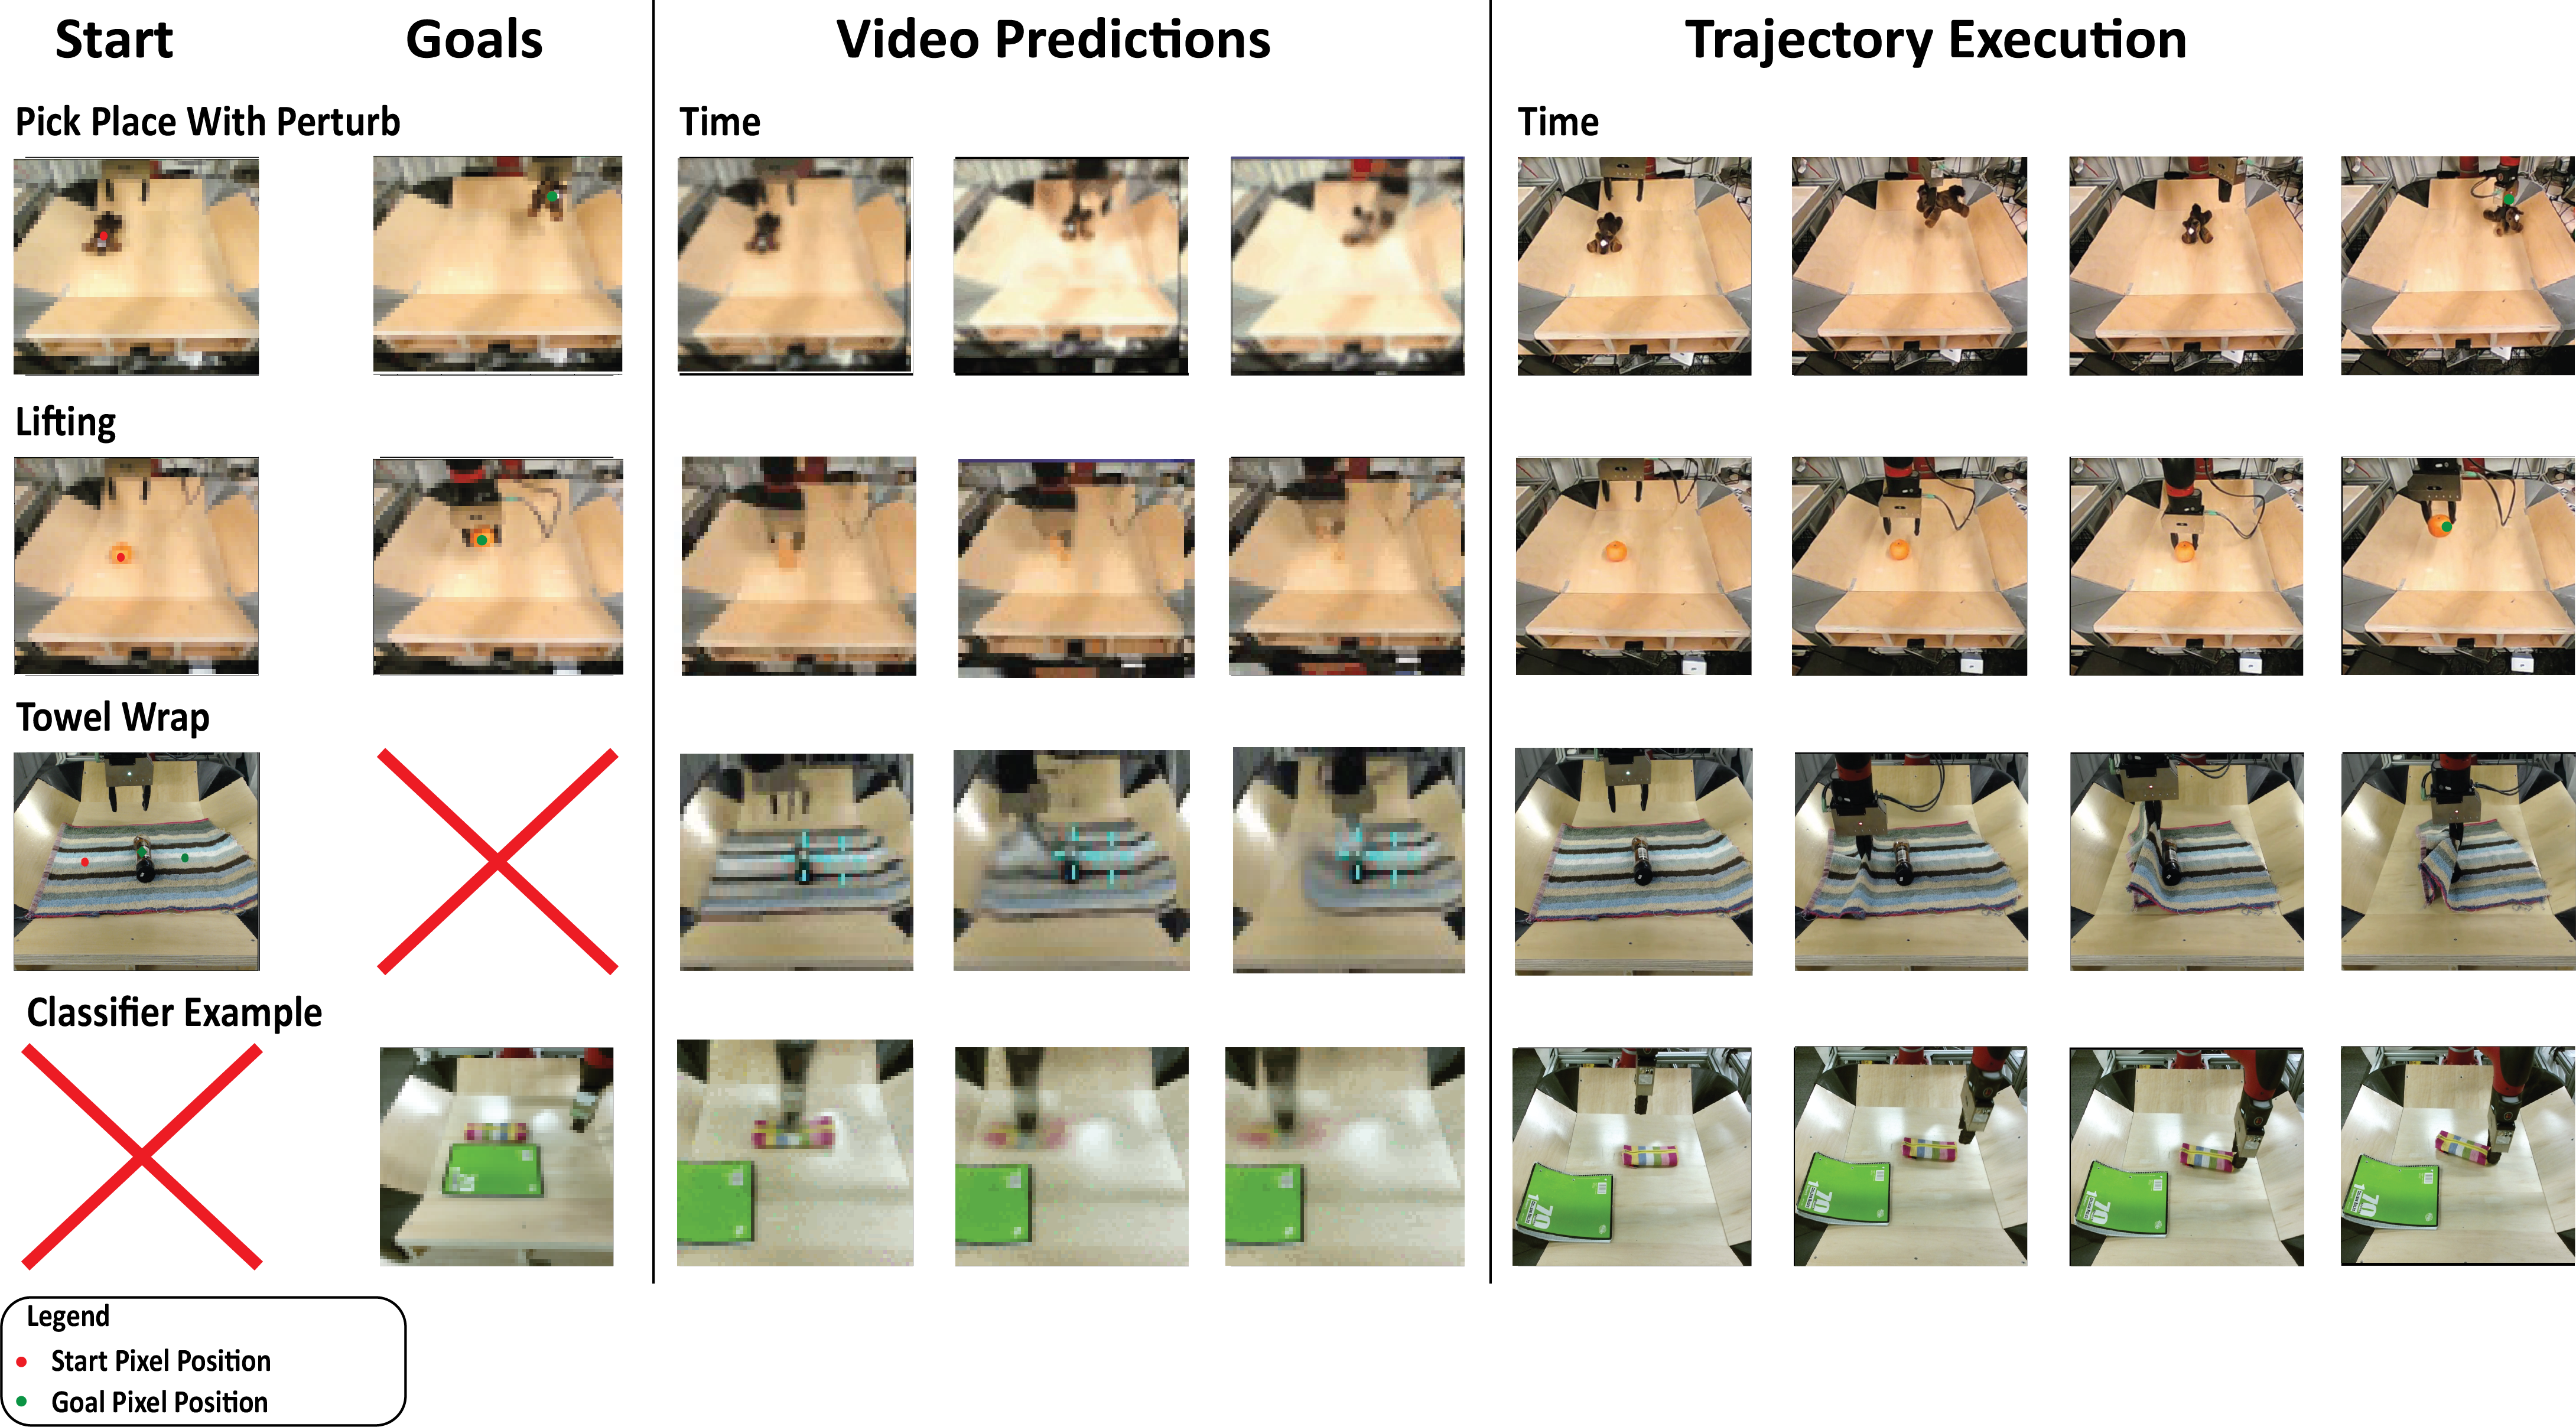
\includegraphics[width=1\columnwidth,trim={0mm 0 0 0},clip]{images_general/tile_rough.png}
	\caption{Visual MPC generalizes to a wide range of tasks and objects, allowing flexibility in goal specification and both rigid and deformable objects not seen during training. Each row shows a different example trajectory. From left to right, we show the task definition, the video-predictions for the planned motion, and the actual executions. Here a task is defined by moving an object marked by a designated pixel, shown by a red dot to a goal position shown by a green dot. A goal-image with the desired goal-configuration can be provided both in combination with a designated pixel or instead of it. Best viewed in PDF.}
	\label{fig:example_traj}
\end{figure}
We approach the problem of learning generalizable behavior in the real world from the standpoint of sensory prediction. Prediction is often considered a fundamental component of intelligence. If we predict raw sensory observations directly, we do not need to assume availability of low-dimensional state information or an extrinsic reward signal. Through prediction, it is possible to learn useful concepts about the world even from a raw stream of sensory observations, such as images from a camera. Image observations are both information-rich and high-dimensional, presenting both an opportunity and a challenge. Future observations provide a substantial amount of supervisory information for a machine learning algorithm. However, the predictive model must have the capacity to predict these high-dimensional observations, and the control algorithm must be able to use such a model to effectively select actions to accomplish user-specified goals.  Examples for the user-specified goals we consider are shown in figure \ref{fig:example_traj}.
%%CF.11.04:  Need a transition from this paragraph to the next.
%%SL.11.11: I gave it a shot


%Instead of focusing on mastery of highly-specialized skills in closed-world environments, here we focus on \emph{generalization} in diverse environments.
%%SL.09.03: this is an important and critical sentence, but I don't like that we from the outset present it in contrast to something so negative (those other guys fail at this, but we don't) -- just say what we do well, and then talk about alternatives. I think we can motivate the work and explain the challenge without necessarily getting so bogged down in the failure of prior work.
We study control via prediction in the context of robotic manipulation, formulating a model-based reinforcement learning approach centered around prediction of raw sensory observations. One of the biggest challenges in learning-based robotic manipulation is generalization: how can we learn models that are useful not just for a narrow range of tasks seen during training, but that can be used to perform new tasks with new objects that were not seen previously?
Collecting a training dataset that is sufficiently rich and diverse is often challenging in highly-structured robotics experiments, which depend on human intervention for reward signals, resets, and safety. We instead set up a minimally structured robotic control domain, where data is collected by the robot via unsupervised interaction with a wide range of objects, making it practical to collect large amounts of interaction data. The robot collects a stream of raw sensory observations (image pixels), without any reward signal at training time, and without the ability to reset the environment between episodes. This setting is both realistic and necessary for studying RL in diverse real-world environments, as it enables automated and unattended collection of diverse interaction experience. Since the training setting affords no readily accessible reward signal, learning by prediction presents an appealing option: the supervision signal for prediction is always available even in the stream of unsupervised experience.
We therefore propose to learn action-conditioned predictive models directly on raw pixel observations, and show that they can be used to accomplish a range of pixel-based manipulation tasks on a real robot in the physical world at test-time. 

%%CF.11.04: Deleted the below since it seemed repetitive
%Sensory prediction models are goal-agnostic, which enables learning for a variety of different goals at the same time. 
%By learning from raw sensor readings, they are also fully general, in that they do not require access to any other state representation beyond the observations. %%CF: This above sentence is repetitive 
%Our overall approach amounts to a deep model-based reinforcement learning algorithm that leverages video prediction models to perform a variety of pixel-based control tasks.
%In addition the practicality of leveraging the only available supervision in such sparse reward environments, sensory prediciton models are also goal-agnostic, which enables learning for a variety of different goals.
%% TODO - motivate why not to learn a model on top of a more abstract representation of the observations? [The supervision, inherently, comes from the same place.]
%TODO - motivate why raw pixels rather than more compact representation (because pixels contain complete information -- can give Sergey's crossing-the-street example -- and pixels are the only thing that is readily available; also pixels contain more supervision)
%Despite the benefits, a number of challenges arise when aiming to use sensory prediction models: how can we learn a model of high-dimensional observations, and how should an objective or reward be determined with respect to the predicted observations? %how should experience be collected? %how should actions be chosen with respect to the model?
%We discuss each of these design decisions and propose several options, weighting the benefits and trade-offs of each.
%Our overall approach amounts to a deep model-based reinforcement learning algorithm that leverages video prediction models to achieve a variety of pixel-based control tasks without shaped reward information.
The main contributions of this work are as follows. We present \emph{visual MPC}, a general framework for deep reinforcement learning with sensory prediction models that is suitable for learning behaviors in diverse, open-world environments (see figure~\ref{fig:overview}).
We describe deep network architectures that are effective for predicting pixel-level observations amid occlusions and with novel objects. Unlike low-dimensional representations of state, specifying and evaluating the reward from pixel predictions at test-time is nontrivial: we present several practical methods for specifying and evaluating progress towards the goal---including distances to goal pixel positions, registration to goal images, and image classifiers---and compare their effectiveness and use-cases.
%, abstracting away the model architecture %, the policy optimization, 
%and the form of the reward function with respect to predicted observations.
Finally, our evaluation shows how these components can be combined to enable a real robot to perform a range of object manipulation tasks from raw pixel observations. Our experiments include manipulation of previously unseen objects, handling multiple objects, pushing objects around obstructions, handling clutter, manipulating deformable objects such as cloth, recovering from large perturbations, and grasping and maneuvering objects to user-specified locations in 3D-space. These results represent a significant advance in the \emph{generality} of skills that can be acquired by a real robot operating on raw pixel values using a single model.

This article combines and extends material from several prior conference papers~\cite{foresight,sna,ebert2018robustness,flo}, presenting them in the context of a unified system. We include additional experiments, including cloth manipulation and placing tasks, a quantitative \emph{multi-task benchmark} assessing the performance of our method on a wide range of tasks, as well as a comprehensive, open-sourced simulation environment to facilitate future research and better reproducibility. The code and videos can be found on the following webpage\footnote{For videos \& code: \url{https://sites.google.com/view/visualforesight}}.
%%SL.10.15: make sure we actually have all this :)

\begin{figure}[t]
\centering
\includegraphics[width=\columnwidth,trim={0mm 0 0 0},clip]{images_general/overview_roughdraft.png}
\caption{\small{Overview of visual MPC. At training time (top) interaction data is collected autonomously and used to train a video-prediction model. At test time (bottom) this model is used for samnpling-based planning. In this work we discuss three different choices for the planning objective.}}
\label{fig:overview}
\end{figure}




 






% Motivate self-supervised learning
% discuss relationship with reinforcement learning

\section{Related Work}\label{sec:rel_work}

\subsection{Reinforcement Learning with external reward signals}
While reinforcement learning \emph{reinforces} good behavior our approach learns a \emph{goal-agnostic} model that can be used across a wide range of tasks, not known at training time.

\subsection{Large-Scale, Self-Supervised Robotic Learning}

In a number of recent works large-scale robotic data collection (often using multiple robots) has been the key factor enabling the automatic acquisition of generalizable features and skills. Several prior works have focused on autonomous data collection for individual skills, such as grasping~\cite{lerrel,google_handeye} or obstacle avoidance~\cite{greg_kahn_uncertainty,crashing}. In contrast to these methods, our approach learns predictive models that can be used to perform a variety of manipulations, and does not require a success measure or reward function during data collection. 

In \cite{pulkit} Agrawal et al. propose learning an inverse model from raw sensory data without any supervision. While these methods demonstrated effective generalization to new objects, they were limited in the complexity of tasks and time-scale at which these tasks could be performed. The method was able to plan single pokes, and then greedily execute multiple pokes in sequence. We observe a substantial improvement in the length and complexity of manipulations that can be performed with our method.

%Thanard's model:
Kurutach et al. use a InfoGAN model \cite{kurutach2018learning} to learn a latent-space describing the environment states in which planning can be performed. The model can be used to obtain a sequence of waypoints in the latent space between the current state and goal-state. The method currently relies on an inverse model to reach the states proposed by the InfoGAN model. So far experiments have been limited to rope rearrangement tasks.

\subsection{Sensory Prediction Models}
We propose to leverage sensory prediction models, in particular video-prediction, to achieve large-scale self-supervised learning. Relevant related work on video-prediction has been carried out in the context of synthetic video game images~\cite{atarioh,recurrentsimulators} and robotic manipulation~\cite{bootsetal,finn_nips,video_pixel_networks}. Video prediction without actions has been studied for unstructured videos~\cite{beyond_mse,convlstm,vondrick} and driving~\cite{prednet,dynamic_filter_networks}. Several works have sought to use more complex distributions for future images, for example by using autoregressive models~\cite{video_pixel_networks,scott_reed}. While this often produces sharp predictions, the resulting models are extremely demanding computationally which would be impractical for real-world robotic control. In this work, we extend video prediction methods that are based on predicting a transformation from the previous image~\cite{finn_nips,dynamic_filter_networks}. Prior work has also sought to predict motion directly in 3D, using 3D point clouds obtained from a depth camera~\cite{se3}, requiring point-to-point correspondences over time, which makes it hard to apply to previously unseen objects. Our predictive model is effective for a wide range of real-world object manipulations and does not require 3D depth sensing or point-to-point correspondences between frames.


% discuss related work on video-prediction
% on model-predictive control (e.g. Anusha's work)
% visual servoing
% environment modeling e.g. interaction networks

\section{Visual Model Predictive Control}\label{sec:prelim}
\label{sec:vmpc}
%%SL.10.15: change title to Overview?

%%SL.10.15: This is the wrong level of abstraction for this section. This section should provide a high-level overview of the structure of the method: data collection (how is that done?), model training, some considerations about the model (what is input and what is output?) and a brief summary of the test-time control method, not at the level of designated pixels yet, but maybe with a short summary of different ways to specify costs and some details about planning. I recommend starting with a high level motivation sentence or two, and then having \textbf{} paragraph headings for "Training data collection" "Model training" and "Test-time control", then briefly summarize what the following sections will be about, something like "In the next section, we will discuss the architectures and training procedures for our predictive models, followed by a discussion of planning objectives in Section~\ref{sec:something}, planning in Section~\ref{sec:something}, and system design considerations in Section~\ref{sec:something}." Here is an example for how you can open with the high level motivation: In this section, we summarize our visual model-predictive control (MPC) approach, which consists of a model-based reinforcement learning approach to end-to-end learning of robotic manipulation skills. Our method consists of three phases: unsupervised data collection, predictive model training, and planning-based control via the model at test-time.
In this section, we define the visual model-predictive control (MPC) problem formulation.  We assume that the user defines a goal in terms of pixel motion by clicking on the object in the image and a corresponding target location, or by providing one or several demonstrations. Designated pixel positions and demonstrations can also be combined. Based on either of these task definitions we define per-time step cost functions $c_t$ which are computed based on the results of the \emph{action-conditioned} video-prediction model. To find an action sequence $a_{t_0:T}$ for which $c = \sum^{T}_{t=t_0}{c_t}$ over the time steps is minimal we use sampling based planning: A large number of candidate action sequences is sampled and the model's predictions are evaluated using $c$. The first action of the sequence which achieved lowest cost is applied to the robot.

To render the planning process more efficient we use the cross-entropy method (CEM), a gradient-free optimization procedure that consists of iteratively resampling action sequences and refitting Gaussian distributions to the actions with the best predicted cost. Further details can be found in section \ref{sec:optimizer}.

To improve robustness against imperfect models, the actions are iteratively replanned at each real-world time step $\tau \in \{0,...,\tau_{max}\}$ following the framework of model-predictive control (MPC): at each real-world step\footnote{With real-world step we mean timestep of the real-world as opposed to predicted timesteps.} $\tau$, the model is used to plan $T$ steps into the future, and the first action of the plan is executed.





% explain the idea of model-based RL
% explain MPC
% explain shooting methods

\section{Video Prediction for Control}
\label{sec:model}

\begin{figure}[t]
	\centering
	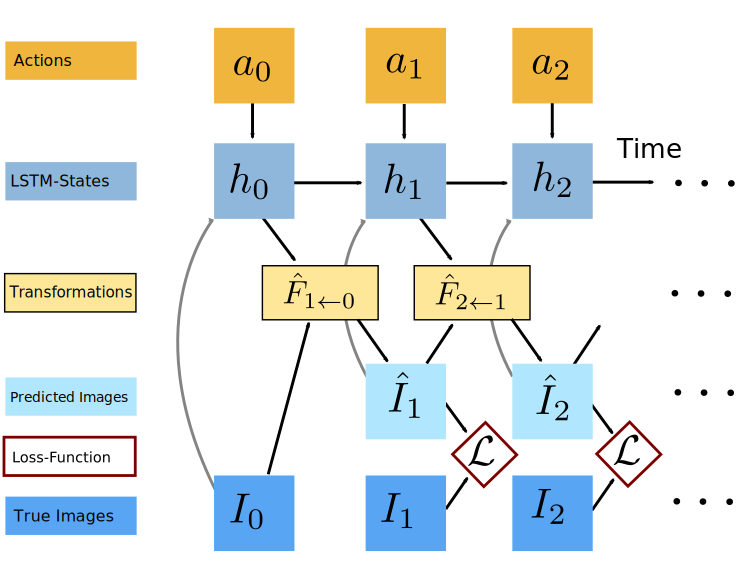
\includegraphics[width=0.7\columnwidth]{images_general/prediction_model.pdf}
	\caption{\small{Computation graph of the video-prediction model. Time goes from left to right, $a_t$ are the actions, $h_t$ are the hidden states in the recurrent neural network, $\hat{F}_{t+1 \leftarrow t}$ is a 2D-warping field, $I_t$ are real images, and $\hat{I}_t$ are predicted images, $\mathcal{L}$ is a pairwise training-loss. \todo{update this}}}   
	\label{fig:prediction_model}
\end{figure}

In visual-MPC we use a transformation-based video-prediction architecture, first presented in \cite{finn_nips}. The advantage of using transformation based-models over a model that directly generates pixels, is that prediction is easier when only few objects in the image move by relatively small amounts and also the transformations can be leveraged to obtain predictions of \emph{where} certain pixels in the image are moving, a property that is used in several of our planning cost-function formulations. The model, which is implemented as a recurrent neural network $g_{\theta}$ parameterized by $\theta$, has a hidden state $h_t$ and takes in a previous image and an action at each step of the rollout. Future images $\hat{I}_{t+1}$ are generated by warping the previous generated image $\hat{I}_t$ or the previous true image $I_t$, when available, according to a 2-dimensional flow field $\hat{F}_{t+1 \leftarrow t}$. A simplifying illustration of model's structure is given in figure \ref{fig:prediction_model}. It is also summarized in the following two equations:

\begin{align}
[h_{t+1}, \hat{F}_{t+1 \leftarrow t}] 	&= g_{\theta}(a_t, h_t, I_t) \\
\hat{I}_{t+1} 							&= \hat{F}_{t+1 \leftarrow t} \diamond  \hat{I}_t 
\label{simple_dna}
\end{align}

Here bilinear sampling operator $\diamond$ interpolates the pixel values bilinearly with respect to a location $(x,y)$ and its four neighbouring pixels in the image, similar to \cite{zhou2016view}. Note that as shown in figure \ref{fig:prediction_model}, at the first time-step the real image is transformed, whereas at later timesteps previously generated images are transformed. The model is trained by standard backpropagtion-through time by performing gradient descent on a mean-squared error type image reconstruction loss, denoted by $\mathcal{L}$ in figure \ref{fig:prediction_model}.
\begin{figure}[t]
    \centering
    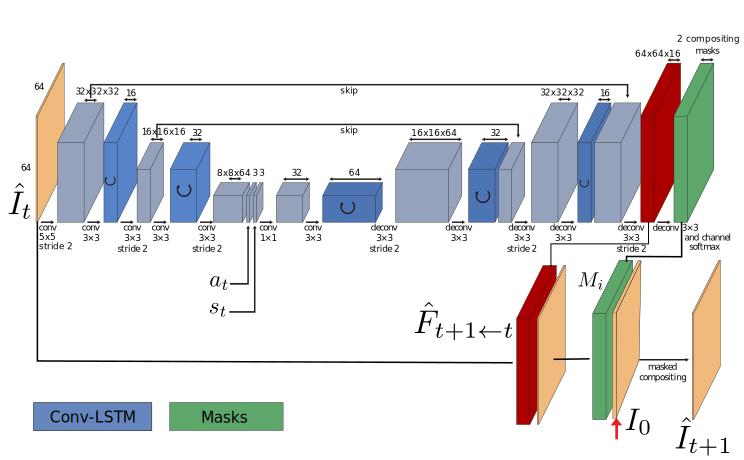
\includegraphics[width=\columnwidth]{images_sna/occlusionaware/architecture.pdf}
    \caption{\small{Forward pass through the recurrent SNA model based on \autoref{eqn:simplemodel}. The red arrow indicates where the image from the first time step $I_0$ is concatenated with the transformed images $\hat{F}_{t+1 \leftarrow t} \diamond  \hat{I}_t $ multiplying each channel with a separate mask to produce the predicted frame for step $t+1$.}}      \label{fig:occlusion_model}
\end{figure}

\label{subsec:pixel_trafo}
A forward pass of the RNN is illustrated in figure \ref{fig:occlusion_model}. We use a series stacked convolutional LSTMs and standard convolutional layers interleaved with average-pooling layers. The result of this computation is the 2 dimensional flow-field $\hat{F}_{t+1 \leftarrow t}$ which is used to transform a current image $I_t$ or $\hat{I}_t$.

\textbf{Predicting motion of individual pixels}: 
When using visual-MPC with a cost-function based on start- and goal pixel positions, a model is required that can effectively predict the 2-D motion of the user-selected start pixels $\pixel_0^{(1)}, \dots, \pixel_0^{(P)}$ up to $T$ steps into the future. Since the model we employ is transformation based, this motion prediction capability emerges implicitly, and therefore no external pixel motion supervision is required. To predict the future positions of the designated pixel $d$, the same transformations which are used to transform the images are applied to the distribution over designated pixel locations. The warping transformation $\hat{F}_{t+1 \leftarrow t}$ can be interpreted as a stochastic transition operator allowing us to make probabilistic predictions about future locations of individual pixels:

\begin{equation}
\hat{P}_{t+1} = \hat{F}_{t+1 \leftarrow t} \diamond  \hat{P}_t
\label{eqn:prob_forward}
\end{equation}

Here $P_t$ is a distribution over image locations which has the same spatial dimension as the image. For simplicity we assume that we only use a single designated pixel. At the first time step the distribution $\hat{P}_0$ is defined as 1 at the position of the user-selected designated pixel and zero elsewhere. The distribution $\hat{P}_{t+1}$ is normalized at each prediction step.

Since this basic model, which we refer to as dynamic neural advection (DNA) model, predicts images only based on the previous image, it is unable to recover shapes (e.g., objects) after they have been occluded, for example by the robot arm. Therefore, this model is only suitable for planning motions where the user-selected pixels are not occluded during the manipulation, which restricts its use in cluttered environments or with multiple selected pixels. In the next section, we introduce an enhanced type of model, which lifts this limitation by employing temporal skip connections.

Note that when using a planning cost function that does not depend on the prediction of pixel positions, like a classifier-based cost function, as detailed in section \ref{subsec:class_cost}, we do not require the model to output transformations and virtually any video prediction model can be used. 

\textbf{Skip Connection Neural Advection Model}
To enable effective tracking of objects through occlusions, we can extend the model discussed in the previous section with temporal skip connections: we now transform pixels not only from the previously generated image $\hat{I}_t$, but from all but from all previous images $\hat{I}_1,...\hat{I}_{t}$, including the context image $I_0$, which is a real image. All these transformed images can combined to a form the predicted image $\hat{I}_{t+1}$ by taking a weighted some over all transformed images, where the weights are given by masks $\mathbf{M}_t$ with the same size as the image and a single channel:
\begin{equation}
\hat{I}_{t+1} =  \mathbf{M}_{0} (\hat{F}_{t+1 \leftarrow 0} \diamond I_t) +  \sum_{j=1}^{\tau} \mathbf{M}_{j} (\hat{F}_{t+1 \leftarrow j} \diamond  \hat{I}_j).
\end{equation}

We refer to this model as the \emph{skip connection neural advection model (SNA)}, since it handles occlusions by using temporal skip-connections such that when a pixel is occluded (e.g., by the robot arm or by another object) it can still reappear later in the sequence.

Transforming from all previous images comes with increased computational cost, since the number of masks and transformations scales with the number of time-steps $\tau$. However, we found that in practice a greatly simplified version of this model, where transformations are applied only to the previous image and the \emph{first image} of the sequence $I_0$ works equally well. Moreover we found that transforming the first image of the sequence is not necessary, as the model uses its pixels primarily to generate the image background. Therefore, we can use the first image directly, without transformation, such that
\begin{equation}
\hat{I}_{t+1} = \mathbf{M}_{0} I_0 +  \mathbf{M}_{1} (\hat{F}_{t+1 \leftarrow t} \diamond \hat{I}_t).
\label{eqn:simplemodel}
\end{equation}
Here, we make the assumption that occluded objects are static throughout the prediction horizon. This assumption allows us to dispense the intermediate transformations and only provide a skip connection from the very first image in the sequence $I_0$, which is also the only real image, since all of the subsequent images are predicted by the model. Hence, this model only needs to output 2 masks. 

 \begin{wrapfigure}{r}{.37\columnwidth}
	\centering
	\includegraphics[width=0.37\columnwidth]{images_sna/occlusionaware/img_desigpixb0.png}
	\caption{The blue dot indicates the designated pixel}
	\label{fig:desig_pix_bluedot}
\end{wrapfigure}

We provide an example of the model recovering from occlusion in \autoref{fig:pix_reappear}. In this figure, the arm is predicted to move in front of the designated pixel, marked in blue in \autoref{fig:desig_pix_bluedot}. The predictions of the DNA model, shown in figure \autoref{fig:pix_reappear}(b), contain incorrect motion of the marked object, as shown in the heatmaps visualizing $\hat{P}_t$, although the arm actually passes in front of it. This is because the DNA model cannot recover information about an object that it has `overwritten' during its predictions, causing the model to predict that the pixel \emph{moves with the arm}. We identified this as one of the major causes of planning failure using the DNA model. By contrast our SNA model predicts that the occluded object will not move, shown in figure  \autoref{fig:pix_reappear}(a).

%\todo{can cut from here:}
%Next, we show another illustration comparing the occlusion handling of DNA and the proposed SNA model. The graphs in \autoref{fig:pix_reqppear_graph} show the predicted probability evaluated at the position of the designated pixel, shown in figure \ref{fig:desig_pix_bluedot}, which is stationary during the entire motion. Precisely when the arm occludes the designated pixel, the probability at this point decreases. This indicates that the model is `unsure' where this pixel is. When the arm unoccludes the designated pixel, it should become visible again, and the probability of the designated pixel being at its original position should go up. In the case of the DNA model and its variants~\cite{finn_nips}, the probability mass does not increase after the object reappears. 
% 
% \begin{figure}[t]
% 	\centering
% 	\includegraphics[width=0.9\columnwidth]{images_sna/occlusionaware/probability_curves.pdf}
% 	\caption{Predicted probability $P_{d^{(0)}}(t)$ of the designated pixel being at the location of the blue dot indicated in \autoref{fig:desig_pix_bluedot} for the DNA model (left) and the SNA model (right). \todo{can cut if no more space!}}      \label{fig:pix_reqppear_graph}
% \end{figure}

\begin{figure}
    \centering
    \begin{subfigure}{0.9\columnwidth}
    \centering
        \includegraphics[width=1.\linewidth]{images_sna/occlusionaware/cdna_1ststep_bckgd_gen_pixb0_overtime.png}
        \caption{Skip connection neural advection (SNA) does not erase or move objects in the background}
        \label{fig:Ng1}
    \end{subfigure}
    \begin{subfigure}{0.9\columnwidth}
    \centering
        \includegraphics[width=1.0\linewidth]{images_sna/occlusionaware/orig_dna_gen_pixb0_overtime.png}
        \caption{Standard DNA \cite{foresight} exhibits undesirable movement of the distribution $P_{d}(t)$ and erases the background}
    \end{subfigure}
    \caption{
    %\protect\subref{fig:Ng1} 
    Top rows: Predicted images of arm moving \textit{in front of} green object with designated pixel (as indicated in \autoref{fig:desig_pix_bluedot}). 
    %(\protect\subref{fig:Ng2}) 
    Bottom rows: Predicted probability distributions $P_{d}(t)$ of designated pixel obtained by repeatedly applying transformations.}
    \label{fig:pix_reappear}
\end{figure}

% explain evolution of video-predction models, CDNA, SNA, SAVP

\section{Planning Cost Functions}


\subsection{Pixel-Distance based Cost}
A convenient way to define a robot task is by choosing one or more pixels in the given an image from the robot's camera and choosing a destination where each pixel should be moved. For example, the user might select a pixel on an object and ask the robot to move it 10 cm to the left. Formally, the user specifies $P$ source pixel locations $\pixel_0^{(1)}, \dots, \pixel_0^{(P)}$ in the initial image $I_0$, and $P$ goal locations $\goal^{(1)}, \dots, \goal^{(P)}$. The source and goal pixel locations are denoted by the coordinates $(x_d^{(i)}, y_d^{(i)})$ and $(x_g^{(i)}, y_g^{(i)})$. Given a goal, the robot plans for a sequence of actions $\action_{1:T}$ over $T$ time steps, where $T$ is the planning horizon. For this type of task definition the problem is formulated as the minimization of a cost function $c$ which depends on the predicted pixel positions $d_t^{(j)}$. The planner makes use of a learned model that predicts a distribution over the pixel position by internally predicting pixel transformations. Given a distribution over pixel positions $P_{t_0, d^{(i)}}\in\mathbb{R}^{H\times W}, \sum_{H,W} P_{t_0, d^{(i)}} = 1$ at time $t = 0$, the model predicts distributions over its positions $P_{t, d^{(i)}}$ at time $t \in \{ 1, \dots, T \}$. The optimizer then finds the action sequence $a_{t_0:T}$ for which the sum of the costs $c_t$ over the time steps is minimal. $c_t$ is defined as the expected euclidean distance between to the goal point $g^{(i)}$.

The expetecd distance to the goal provides smoother planning objective that makes used of the uncertainty estimates of the predictor enabling complex, longer-horizon tasks. This cost function encourages the movement of the designated objects in the right direction for each step of the execution, regardless of whether the $\goal$ position can be reached within $T$ time steps. For multi-objective tasks with multiple designated pixels $d^{(i)}$ the costs are summed to together weighting them equally.



In subsequent steps ($\tau > 0$), the 1-step ahead prediction of the previous step is used to initialize $P_{t=0,d^{(i)}}$. 

\subsection{Registration-based Cost}



\subsection{Classifier-based Cost}
\label{subsec:class_cost}



% pixel distance based costs
% registration based costs
% combination of registration based cost with pixel distance cost
% classifier based costs

\section{Trajectory Optimizer}

\begin{algorithm}[ht]
\caption{Planning in Visual MPC}
\label{alg:opt}
\begin{algorithmic}[1]
\State \textbf{Inputs:} Predictive model $g$, planning cost function $c$
\For{$t~=~0...T-1$}

\For{$i~=~0...n_{iter}-1$}
\If{$i==0$}
\State \begin{varwidth}[t]{\linewidth}
	Sample $M$ action sequences $\{a^{(m)}_{t:t+H-1}\}$ from \par $\mathcal N(0, I)$ or
	custom sampling distribution
\end{varwidth}
\Else
\State \begin{varwidth}[t]{\linewidth}
	Sample $M$ action sequences ${a^{(m)}_{t:t+H-1}}$ from \par 
	$\mathcal N(\mu^{(i)}, \Sigma^{(i)})$
\end{varwidth}
\EndIf
\State 
\begin{varwidth}[t]{\linewidth}
Check if sampled actions are within \par
admissible range, otherwise resample.
\end{varwidth}
\State  \begin{varwidth}[t]{\linewidth}
	Use $g$ to predict future  image sequences $\hat{I}_{t:t+H-1}^{(m)}$\\ and probability distributions $\hat{P}_{t:t+H-1}^{(m)}$
\end{varwidth}
\State Evaluate action sequences using a cost function $c$
\State  \begin{varwidth}[t]{\linewidth}
	Fit a diagonal Gaussian to the $k$  action samples\\ with lowest cost,
	yielding $\mu^{(i)}, \Sigma^{(i)}$
\end{varwidth}
\EndFor
\State Apply first action of best action sequence to robot
\EndFor
\end{algorithmic}
\end{algorithm}


\label{sec:optimizer}
The role of the optimizer is to find actions sequences $a_{1:T}$ that minimize the sum of the costs $c_{1:T}$ along the planning horizon $T$. We use a simple stochastic optimization procedure for this, based on the cross-entropy method (CEM), a gradient-free optimization procedure. CEM consists of iteratively resampling action sequences and refitting Gaussian distributions to the actions with the best predicted cost.

Although a variety of trajectory optimization methods may be suitable, one advantage of the stochastic optimization procedure is that it allows us to easily ensure that actions stay within the distribution of actions the model encountered during training. This is crucial to ensure that the model does not receive out-of-distribution inputs and makes valid predictions.  Algorithm \ref{alg:opt} illustrates the planning process. In practice this can be achieved by defining admissible ranges for each dimension of the action vector and rejecting a sample if it is outside of the admissible range. 

In the appendix \ref{sec:cem_improv} we present a few improvements to the CEM optimizer for visual MPC.
%%SL.11.21: This paragraph confuses me. How does gradient-free stochastic optimization constrain the optimizer to stay within the distribution of training states? Without any explanation of a mechanism, this paragraph is not very convincing. My suggestion would be to either list different reasons for using CEM, or provide a more convincing justification.
% explain the cross entroy method
% explain reusing actions

\section{System Design}
\begin{figure}
	\centering
	\includegraphics[width=1.0\linewidth]{images_general/robot_setup.jpg}
	\caption{\small{Robot setup, with 2 standard web-cams arranged at different viewing angles.}
		\label{fig:robot_setup}
	}
\end{figure}
\label{sec:system}

In this section we explain our robot setup and several critical system design choices and details about the data collection process.

\textbf{Learning complex Pick and Place Behavior:}
When collecting data by sampling from simple distributions, such as multivariate Gaussian, the skills that emerged were found to be generally restricted to pushing and dragging objects. This is because with simple distributions, it is very unlikely to visit states like picking up and placing of objects or folding cloth. Not only would the model be imprecise for these kinds of states, but also during planning it would be unlikely to \emph{find} action sequences that grasp an object or fold. 
We therefore explore how the sampling distribution used both for data collection and sampling-based planning can be changed to visit these, otherwise unlikely, states more frequently, allowing more complex behavior to emerge. 

We first discuss picking and placing of objects. To allow picking up and placing of objects to occur more frequently, we incorporate a simple ``reflex'' during data collection, where the gripper automatically closes, when the height of the wrist above the table is lower than a small threshold. This reflex is inspired by the palmar reflex observed in infants~\cite{grasping_fetal}. With this primitive, about 20\% of training trajectories included some sort of grasp on an object. It is worth noting that, other than this reflex, no grasping-specific engineering was applied to the policy allowing a joint pushing and grasping policy to emerge, see figure \ref{fig:push_grasp}. In our experiments, we evaluate our method using data obtained both with and without the grasping reflex, evaluating both purely non-prehensile and combined prehensile and non-prehensile manipulation.


%%SL.10.15: Have transition here and explain what this section is about. Currently, it seems like a bunch of disjointed miscallaneous stuff that didn't fit in anywhere else. This is not good. Maybe you can call this system design and describe the robot setup here first (both single view and multi-view), then details about data collection -- how actions are selected etc. (which can be merged with 7.2). Figures would help to illustrate the robot setup. 7.3 probably doesn't belong here at all, but belongs in experiments

The visual MPC algorithm as described so far is only able to solve manipulation tasks specified in 2D, like rearranging objects on the table, however a task such as lifting an object to a particular position in 3D cannot be fully specified with a single view, since it would be ambiguous. 

\textbf{Multi-view visual MPC:} We use a combination of multiple views, taken with multiple cameras arranged appropriately, to jointly define a 3D task. Figure \ref{fig:robot_setup} shows the robot setup, including 2 standard webcams observing the workspace from different angles. The registration method described in the previous section is used separately per view to allow for dynamic retrying and solving temporally extended tasks. The planning costs from each view are combined using weighted averaging where the weights are provided by the registration network (see equation \ref{eqn:cost_avg}).  \todo{Figure XX shows an example lifting task, which specified in two views.}

The classifier-based cost is also used in the multiview-setup, an example trajectory of cloth folding is shown \todo{in figure}. 






\section{Experimental Evaluation}
\label{sec:experiments}

Our experimental evaluation consists of three parts, each answering one of the following three questions:
\begin{itemize}
	\item How does a smooth cost function 
	\item How does the skip-connection neural advection model compare to 
\end{itemize}


%%SL.10.16: It would help to add a transition here. Discuss the goals of the experiments and provide a short overview for the reader, so that none of the experiment subsections come as a surprise.

%%SL.10.16: Put all these boring details into some subsection titled something like Experimental Setup. However, a lot of this is actually supposed to be covered in Section 7 above -- it's a bit weird to have a bunch more experimental setup now in this section. Maybe try to collect it all in one place?
To train both our video-prediction and registration models, we collected 20,000 trajectories of pushing motions and 15,000 trajectories with gripper control, where the robot was allowed to randomly move and pick up objects. The data collection process is fully autonomous, requiring human intervention only to replace and change out the objects in front of the robot.

The action space consisted of Cartesian movements along the $x$, $y$, and $z$ axes, and for some parts of it we also added azimuthal rotations of the gripper. For evaluation, we selected novel objects that were never seen during training. The evaluation tasks required the robot to move objects in its environment from a starting state to a goal configuration, and performance was evaluated by measuring the distance between the final object position and goal position. %\todo{how was it done for the classifier?}

\subsection{Evaluating Skip-connection Neural Advection}
\label{subsec:sna_experiments}
\begin{wrapfigure}{r}{.37\columnwidth}
	% \vspace{-0.25in}
	\centering
	\includegraphics[width=0.30\columnwidth]{images_sna/longdistance_pushing/pushing.pdf}
	\caption{
		Pushing task. The designated pixel (red diamond) needs to be pushed to the green circle.
		\label{fig:long_distance_task}
	}
\end{wrapfigure}

We first perform a quantitative comparison of visual-MPC using the proposed
%%SL.10.16: Let's just say that this section is comparing different video prediction models, instead of saying that it's evaluating "our" proposed model
occlusion-aware SNA video prediction model and the expected distance cost with visual-MPC using the dynamic neural advection model (DNA)\cite{foresight} with both the goal-point evaluation cost \ref{eq:goal_point_eval} and the expected distance cost \ref{eq:cost}.
%%SL.10.16: again, just say we're comparing different cost specification methods from Section whatever

We evaluate long pushes and multi-objective tasks where one object must be pushed without disturbing another.
%%SL.10.16: This sounds really disappointing. Presumably we do lots of other cool stuff too? What about classifier, towels, rearrangement and placing tasks?
The supplementary video and links to the code and data are available at \url{https://sites.google.com/view/sna-visual-mpc}

%%SL.10.16: do we use the same test procedure in other subsections too? If so, let's have a separate subsection to describe the experiment, and then separate subsections for results, otherwise there will be a lot of duplication. Don't just staple the experiment sections from different papers together...
\autoref{fig:long_distance_task} shows an example task for the pushing benchmark.
%%SL.10.16: I think these "bare bones" pictures with no distractors are really boring. Can we mostly show interesting tasks with lots of distractors, and contain the simple pushing tasks in one subsection? If we have lots of pictures of the simple tasks, people will conclude that the method only works with one object in the scene.
We collected 20 trajectories with 3 novel objects and 1 training object. \autoref{table:res_dna_sna} shows the results for the pushing benchmark. The column \textit{distance} refers to the mean distance between the goal pixel and the designated pixel at the final time-step. The column \textit{improvement} indicates how much the designated pixel of the objects was moved closer to their goal (or further away for negative values) compared to the starting location. The true locations of the designated pixels after pushing were annotated by a human labeler.

The results in \autoref{table:res_dna_sna} show that our proposed planning cost in \autoref{eq:cost}
%%SL.10.16: wait, what? I thought this section was evaluating models, not costs? Can we separate these out, first evaluate models, then costs, to reflect the organization in the paper?
substantially outperforms the planning cost used in prior work~\cite{foresight}. The performance of the SNA model in these experiments is comparable to the DNA model~\cite{foresight} when both use the expected-distance planning cost, since this task does not involve any occlusions.
%%SL.10.16: Hmm... OK, perhaps if we're going to evaluate costs and models simultaneously like this, we need to organize the sections more clearly. Maybe it would really help in that case to separate out experiment setup (how the methods care compared) from the results (how they stack up). And for each section, ask yourself: what is the question these experiments are trying to answer? It should be obvious from the writing. Right now, I feel like the experiments section looks too much like experiments sections from different papers stapled together. They need to more integrated and focused on achieving the paper's aims: state the research questions, and explain how each experiment subsection answers one or more of those questions
\begin{figure*}
\centering
\includegraphics[width=1\linewidth]{images_sna/multiobject_qualitative/avoid_obstacle.pdf}
\caption{Left: Task setup with green dot marking the obstacle. Right, first row: the predicted frames generated by SNA. Second row: the probability distribution of the designated pixel on the \textit{moving} object (brown stuffed animal). Note that part of the distribution shifts down and left, which is the indicated goal. Third row: the probability distribution of the designated pixel on the obstacle-object (blue power drill). Although the distribution increases in entropy during the occlusion (in the middle), it then recovers and remains on its original position.
\label{fig:goingaroundocclusion}}
\end{figure*}

\begin{table}
{\footnotesize
    \begin{center}
    \begin{tabular}{lcc}
    	\toprule
           &  \thead{dist. \\ $\pm$ std err. of mean} & \thead{improvement \\ $\pm$ std err. of mean}  \\  
           \midrule
      DNA with cost eqn. \ref{eq:goal_point_eval}\cite{foresight}  & 24.6$\pm$2.35 & 2.1$\pm$ 2.75\\
      DNA with cost eqn. \ref{eq:cost}  & \textbf{17.5 $\pm$ 2.37} &  \textbf{8.3 $\pm$ 2.62}\\ 
      SNA with cost eqn. \ref{eq:cost} (ours) & 18.18 $\pm$ 2.1 & 7.7 $\pm$ 2.33\\
      \bottomrule
    \end{tabular}
    \end{center}
    }
    \caption{Results of the pushing benchmark on 20 different object/goal configurations. Units are pixels in the 64x64 images.}
    \label{table:res_dna_sna}
\end{table}


\begin{table}
\centering
{\footnotesize
\begin{tabular}{lcc}
	\toprule
         &  \thead{moved imp. \\ $\pm$ std err. of mean} &   \thead{stationary imp. \\ $\pm$ std err. of mean}  \\
         \midrule
  DNA \cite{foresight} & 0.83 $\pm$0.25 &  -1.1 $\pm$ 0.2\\ 
  SNA & \textbf{10.6 $\pm$ 0.82} & \textbf{-1.5 $\pm$ 0.2} \\
  \bottomrule
\end{tabular}
}

\caption{Results for multi-objective pushing on 8 object/goal configurations with 2 seen and 2 novel objects. Values indicate improvement in distance from starting position, higher is better. Units are pixels in the 64x64 images.} 
\label{table:mult_obj}

\end{table}

%The pushing task evaluates the ability of each method to push an object across the table, but does not explicitly study the effect of occlusions. 
To examine how well each approach can handle occlusions, we devised a second task that requires the robot to push one object, while keeping another object stationary. When the stationary object is in the way, the robot must move the goal object around it, as shown in \autoref{fig:goingaroundocclusion} on the left. While doing this, the gripper may occlude the stationary object, and the task can only be performed successfully if the model can make accurate predictions through this occlusion. These tasks are specified by picking one pixel on the target object, and one on the obstacle. The obstacle is commanded to remain stationary, by choosing the target position to be at the same location as the initial position. For the target object the destination is chosen on the other side of the obstacle.

We used four different object arrangements, with two training objects and two objects that were unseen during training. We found that, in most of the cases, the SNA model was able to find a valid trajectory, while the DNA model, that is not able to handle occlusion, was mostly unable to find a solution. \autoref{fig:goingaroundocclusion} shows an example of the SNA model successfully predicting the position of the obstacle through an occlusion and finding a trajectory that avoids the obstacle. These findings are reflected by our quantitative results shown in \autoref{table:mult_obj}, indicating the importance of temporal skip connections.
%%SL.10.16: It would help if the experimental conclusion at the end of this section is an answer to  question posed earlier in the experiments. I also think it makes too big of a deal out of the SNA thing -- this is not the SNA paper, we don't need to push on this so hard!

\subsection{Evaluating Closed-Loop Visual MPC}
%%SL.10.16: This is very misleading, all of the experiments are closed-loop!

\begin{table}
	{\footnotesize
		\begin{center}
			\begin{tabular}{lcc}
				\toprule
				%				 & \multicolumn{2}{c}{fraction of successful runs} \\
				& Short & Long \\
				\midrule
				Visual MPC $+$ predictor propagation  & 83\% & 20\% \\
				Visual MPC $+$ OpenCV tracking  & 83\%  & 45\% \\
				Visual MPC $+$ registration network & 83\% & \textbf{66\%}  \\
				\bottomrule
			\end{tabular}
		\end{center}
	}
	\caption{\small Success rate for long-distance pushing benchmark with 20 different object/goal configurations and short-distance benchmark with 15 object/goal configurations. Success is defined as bringing the object closer than 15 pixels to the goal, which corresponds to around $7.5cm$.}
	\label{table:res_long_short}
\end{table}

%%SL.10.16: Before talking about videos, explain what this experiment section is actually studying! What is the question? What are you evaluating? Why?
Videos and visualizations for closed-loop visual MPC can be found on this webpage: \url{https://sites.google.com/view/robustness-via-retrying}.
%%SL.10.16: Let's not have multiple different websites. This just confuses the reader. Let's have only one website with results for the journal paper. This is not three papers stapled together, it's a single journal paper, and should be presented as such.
We compare visual-MPC that uses a pixel-distance based cost based on our proposed self-supervised registration with visual-MPC using an off-the-shelf tracker, the ``multiple instance learning tracker'' MIL \cite{babenko2009visual} from OpenCV. Note that all methods do not have any prior knowledge of objects -- it is only provided with the position of one designed pixel in the initial and goal images, and must use the learned model to infer that this pixel belongs to an object that can be moved by the robot.
%%SL.10.16: This is a very strange palce to put this sentence -- doesn't this apply to all experiments?
Finally we also compare to visual MPC without registration method proposed by \cite{sna},
%%SL.10.16: that's this paper!
which does not track the object explicitly, but relies on the flow-based video prediction model to keep track of the designated pixel, which we call ``predictor propagation.'' 
%%SL.10.16: again, that's this paper!

\subsubsection{Pushing with Retrying}
%%SL.10.16: again, not entirely clear what question this is trying to answer

\begin{figure*}
    \centering
    \includegraphics[width=1.0\textwidth]{images_rfr/push_correction.pdf}
    \caption{\small{Applying our method to a pushing task. In the first 3 time instants the object behaves unexpectedly, moving down. The tracking then allows the robot to retry, allowing it to eventually bring the object to the goal.}}
    \label{fig:push_retry}
\end{figure*}


%\begin{figure}
%	\centering
%	\includegraphics[width=0.8\columnwidth]{images_rfr/pushlong_bench_same_range.pdf}
%	\caption{\small{Results for long pushing tasks with 20 objects not seen during training, showing fraction of runs where final distance is lower than threshold. Our method shows a clear gains over OpenCV tracking and predictor propagation.}}
%	\label{fig:push_bench_long}
%\end{figure}

For the first experiment, we disable the gripper control, which requires the robot to push objects to the target.
%%SL.10.16: is this not true in the previous section? can we somehow be a bit more systematic about explaining the experiment setup?
We evaluate our method on 20 long-distance and 15 short-distance pushing tasks. For long-distance tasks the distance between the object and its goal-position is $30cm$ while for short-distance tasks it is $15cm$. Table \ref{table:res_long_short} lists quantitative comparisons showing that on the long-distance benchmark visual-MPC using the proposed registrations approach not only outperforms prior work \cite{sna}, but also outperforms the hand-designed, supervised object tracker \cite{babenko2009visual}. By contrast for the short distance benchmark, all methods perform comparably. Thus theses results indicate the importance of closed loop control in long-horizon tasks. Using our learned registration, the robot is more frequently able to successfully recover after mispredictions or occlusions, an example is shown in \autoref{fig:push_retry}.

%\begin{figure}
%	\centering
%	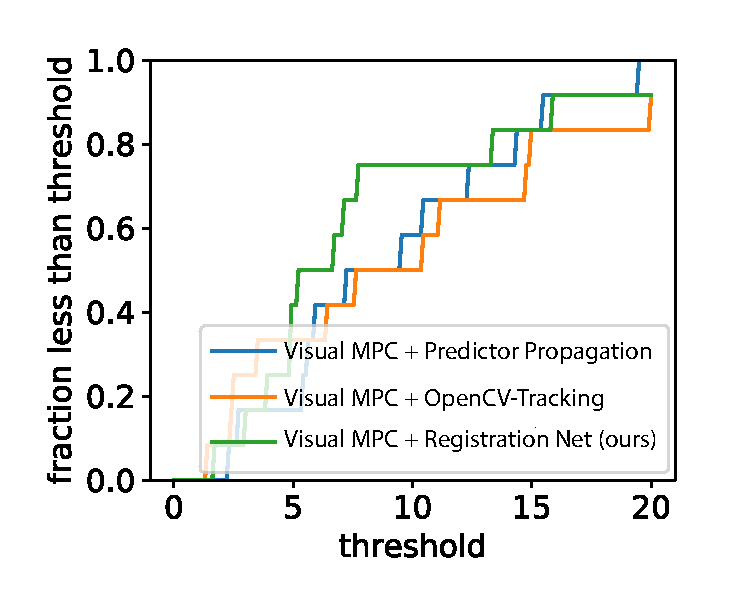
\includegraphics[width=0.8\columnwidth]{images_rfr/pushshort_bench_plots.pdf}
%	\caption{\small{Results for short pushing tasks.  Fraction of runs where final distance is lower than threshold.}}
%	\label{fig:push_bench_short}
%\end{figure}

\subsubsection{Combined Prehensile and Non-Prehensile Manipulation.}
\begin{figure*}
	\centering
	\includegraphics[width=1.0\textwidth]{images_rfr/pick_place_plush.pdf}
	\caption{\small{Retrying behavior of our method combining prehensile and non-prehensile manipulation. In the first 4 time instants shown the robot pushes the object. It then loses the object, and decides to grasp it pulling it all the way to the goal. Retrying is enabled by applying the learned registration to both camera views (here we only show the front view).}}
	\label{fig:push_grasp}
	
\end{figure*}
%%SL.10.16: what is this evaluating?

In the setting where the gripper is enabled it is part of the task to decide whether to solve a task by grasping or pushing the object to the goal. Similarly to the pushing setting we perform a benchmark where we define a set of 20 object relocation tasks and measure the final distance between the object and the target at the end of the episode. Interestingly we observe that in the majority of the cases the agent decides to grasp the object, as can be seen in the supplementary video.
%%SL.10.16: did you mean to reference some table or figure here?

%%SL.10.16: Is there some conclusion to be drawn from all this about different cost functions?

\subsection{Evaluating Classifier-based Cost Function}

For evaluating the performance of the proposed classifier-based cost function, we study a visual object arrangement task, where different goals correspond to different relative arrangements of a pair of objects. 
%We evaluate our learned classifier on the predictions made by the video prediction model \todo{unclear, how exactly do you evaluate the classifier?} and derive the cost used for planning from the predicted probability of success. 

To collect data for meta-training the classifier, we randomly select a pair of objects from our set of training objects, and position them into many different relative positions, recording the image for each configuration. One task corresponds to a particular relative positioning of two objects, e.g. the first object to the left of the second, and we construct positive and negative examples for this task by labeling the aforementioned images. We randomly position the arm in each image, as it is not a determiner of task success. A good objective should ignore the position of the arm. We also include randomly-positioned distractor objects in about a third of the collected images.

We evaluate all approaches in three different experimental settings. In the first setting, the goal is to arrange two objects into a specified relative arrangement. The second setting is the same, but with distractor objects present. In the final, most challenging setting, the goal is to achieve two tasks in sequence. We provide positive examples for both tasks, infer the classifier for both task, perform MPC for the first task until completion, followed by MPC for the second task. To evaluate the ability to generalize to new goals and settings, we use novel, held-out objects for all of the task and distractor objects in our evaluation. Code for training the few-shot goal classifier and videos of our results are available at \url{https://sites.google.com/view/few-shot-goals}.
%%SL.10.16: we should have one website!

We qualitatively visualize the evaluation in Figure~\ref{fig:cls_results}.
%\todo{explain how exactly you measure success} 
On the left, we show a subset of the five images provided to illustrate the task(s), and on the left, we show the motions performed by the robot. We see that the robot is able to execute motions which lead to a correct relative positioning of the objects.
We quantitatively evaluate each method across 20 tasks, including $10$ unique object pairs. The results, shown in Figure~\ref{fig:cls_charts}, indicate that prior methods for learning distance metrics
%%SL.10.16: you mean the method *in this paper*?
struggle to infer the goal of the task, while our approach leads to substantially more successful behavior on average. 

%%SL.10.16: what is the conclusion from all this? how do the different methods of specifying costs stack up?

%%SL.10.16: where are qualitative results and discussion of cloth?

\begin{figure}
    \centering
    \includegraphics[width=0.48\textwidth]{images_cls/cls_charts.jpeg}
    \caption{\small Quantitative performance of visual planning for object rearrangement tasks across different goal specification methods: our meta-learned classifier, DSAE~\cite{finn_nips}, and pixel error. Where possible, we include break down the cause of failures into errors caused by inaccurate prediction or planning and those caused by an inaccurate goal classifier.}
    \label{fig:cls_charts}
    \vspace{-0.3cm}
\end{figure}


\begin{figure*}
    \centering
    \includegraphics[width=0.8\textwidth]{images_cls/cls_results.jpeg}
    \caption{\small Object arrangement performance of our goal classifier with distractor objects and with two tasks. The left shows a subset of the 5 positive examples that are provided for inferring the goal classifier(s), while the right shows the robot executing the specified task(s) via visual planning.}
    \label{fig:cls_results}
    \vspace{-0.3cm}
\end{figure*}

\subsection{Learning Cloth-Folding with Visual-MPC}
\label{subsec:cloth_folding_data}
a major impediment is that when executing random actions clothes can become tangled pu
% pushing benchmark with and without tracking
% grasping
% experiments with stochastic models, optimistic/pessimistic planning



\section{Conclusion}
We presented an algorithm that leverages self-supervision from visual prediction to learn a deep dynamics model on images, and show how it can be embedded into a  planning framework to solve a variety of robotic control tasks. We demonstrate that visual model-predictive control is able to successfully perform multi-object manipulation, pushing, picking and placing, and cloth-folding tasks -- all within a single framework. These tasks involve complex contact dynamics as well as deformable objects, indicating that the same sensory prediction model can be used to capture a wide variety of environment dynamics with enough accuracy to allow for control.

%%SL.10.16: I think the discussion below is not quite a good fit for future work. It's important to understand what the *purpose* of the future work section is. Contrary to what the name might imply, the purpose of future work is *not* to actually discuss future work. The purpose of future work is to inspire the reader that your work has lots of potential to lead to new and exciting research. You should *not* usually talk about immediate next steps you plan to take, but rather all the awesome stuff *enabled* by your work.

%%SL.10.16: What I would recommend is to have one paragraph on limitations (which is actually future work in disguise), and then a future work paragraph meant to inspire the reader about all the great stuff you could do with this method, ending on a very high note in the end about the generality of entirely self-supervised robotic deep model-based RL algorithms.

\noindent \textbf{Limitations}
The main limitations of the presented framework are that all target objects need to be visible throughout execution, it is currently not possible to handle partially observed domains. This is especially important for tasks that require objects to be brought into occlusion (or taken out of occlusion), for example putting an object in a box and closing it. Another limitation is that the tasks are still of only medium duration and usually only touch one or two objects. Longer-term planning remains an open problem. Lastly, the fidelity of object positioning is still significantly below what humans can achieve.

\noindent \textbf{Possible future directions}
The key advantage of a model-based deep-reinforcement learning algorithm like visual MPC is that it \emph{generalizes} to tasks it has never encountered before. This makes visual MPC a good candidate for a building block of future robotic manipulation systems that will be able solve an even wider range of complex tasks with much longer horizons. 


% use section* for acknowledgment
\ifCLASSOPTIONcompsoc
  % The Computer Society usually uses the plural form
%  \section*{Acknowledgments}
\else
  % regular IEEE prefers the singular form
%  \section*{Acknowledgment}
\fi


%The authors would like to thank...The authors would like to thank...The authors would like to thank...The authors would like to thank...The authors would like to thank...The authors would like to thank...The authors would like to thank...The authors would like to thank...The authors would like to thank...The authors would like to thank...


% Can use something like this to put references on a page
% by themselves when using endfloat and the captionsoff option.
\ifCLASSOPTIONcaptionsoff
  \newpage
\fi



% trigger a \newpage just before the given reference
% number - used to balance the columns on the last page
% adjust value as needed - may need to be readjusted if
% the document is modified later
%\IEEEtriggeratref{8}
% The "triggered" command can be changed if desired:
%\IEEEtriggercmd{\enlargethispage{-5in}}

% references section

% can use a bibliography generated by BibTeX as a .bbl file
% BibTeX documentation can be easily obtained at:
% http://mirror.ctan.org/biblio/bibtex/contrib/doc/
% The IEEEtran BibTeX style support page is at:
% http://www.michaelshell.org/tex/ieeetran/bibtex/
%\bibliographystyle{IEEEtran}
% argument is your BibTeX string definitions and bibliography database(s)
%\bibliography{IEEEabrv,../bib/paper}
%
% <OR> manually copy in the resultant .bbl file
% set second argument of \begin to the number of references
% (used to reserve space for the reference number labels box)
% \begin{thebibliography}{1}

% \bibitem{IEEEhowto:kopka}
% H.~Kopka and P.~W. Daly, \emph{A Guide to \LaTeX}, 3rd~ed.\hskip 1em plus
%   0.5em minus 0.4em\relax Harlow, England: Addison-Wesley, 1999.

% \end{thebibliography}

\bibliographystyle{IEEEtran}
\bibliography{mybib}
% biography section
% 
% If you have an EPS/PDF photo (graphicx package needed) extra braces are
% needed around the contents of the optional argument to biography to prevent
% the LaTeX parser from getting confused when it sees the complicated
% \includegraphics command within an optional argument. (You could create
% your own custom macro containing the \includegraphics command to make things
% simpler here.)
%\begin{IEEEbiography}[{\includegraphics[width=1in,height=1.25in,clip,keepaspectratio]{mshell}}]{Michael Shell}
% or if you just want to reserve a space for a photo:
\vskip -13mm

\begin{IEEEbiographynophoto}{Frederik Ebert}
Frederik Ebert received a BS in Mechatronics and Information Technology as well a MS in "Robotics, Cognition, Intelligence (RCI)" from the Technical University of Munich (TUM). He is currently a PhD student at Berkeley Artifical Intelligence Research (BAIR). % institute where he focuses on developing algorithms for robotic manipulation combining ideas from computer vision, machine learning and control.
\end{IEEEbiographynophoto}
\vskip -13mm

% if you will not have a photo at all:
\begin{IEEEbiographynophoto}{Chelsea Finn}
Chelsea Finn is currently a research scientist at Google Brain and a post-doctoral scholar at UC Berkeley. %, and will join the Computer Science faculty at Stanford in 2019. %Her research focuses on algorithms that can enable agents to autonomously learn a range of complex skills. 
She received a BS in Electrical Engineering and Computer Science from MIT and a PhD in Computer Science from UC Berkeley.
\end{IEEEbiographynophoto}
\vskip -13mm

% insert where needed to balance the two columns on the last page with
% biographies
%\newpage

\begin{IEEEbiographynophoto}{Annie Xie}
% Biography text here.
Annie Xie is pursuing a B.S. degree in Electrical Engineering and Computer Science at UC Berkeley. %Her research interests are in the areas of computer vision and robot learning.
\end{IEEEbiographynophoto}
\vskip -13mm

\begin{IEEEbiographynophoto}{Sudeep Dasari}
	Sudeep Dasari is a 4th year student at UC Berkeley pursuing a B.S in Electrical Engineering and Computer Science. %His primary research interests are computer vision, machine learning, and robotic control.
\end{IEEEbiographynophoto}
\vskip -13mm

\begin{IEEEbiographynophoto}{Alex Lee}
	Alex Lee received a BS in Electrical Engineering and Computer Science from UC Berkeley and is currently pursuing a PhD in Computer Science from UC Berkeley. %His work focuses on algorithms that can enable robots to learn complex sensorimotor skills.
\end{IEEEbiographynophoto}
\vskip -13mm

\begin{IEEEbiographynophoto}{Sergey Levine}
Sergey Levine received a BS and MS in Computer Science from Stanford, and a Ph.D. in Computer Science from Stanford. He is currently on the faculty of the Department of Electrical Engineering and Computer Sciences at UC Berkeley. %His work focuses on machine learning for decision making and control, with an emphasis on deep learning and reinforcement learning algorithms.
\end{IEEEbiographynophoto}

% You can push biographies down or up by placing
% a \vfill before or after them. The appropriate
% use of \vfill depends on what kind of text is
% on the last page and whether or not the columns
% are being equalized.

%\vfill

% Can be used to pull up biographies so that the bottom of the last one
% is flush with the other column.
%\enlargethispage{-5in}

\appendices
\newpage

\section{Skip Connection Neural Advection Model}
\label{sec:skipcon}

Our video prediction model, shown in ~\autoref{fig:prediction_model}, is inspired by the dynamic neural advection (DNA) model proposed by~\cite{finn_nips} and it is a variant of the SNA model proposed by~\cite{sna}. The model uses a convolutional LSTM~\cite{convlstm} to predict future frames. The prediction is initialized with an initial sequence of 2 ground truth frames, and predicts 13 futures frames. The model predicts these frames by iteratively making next-frame predictions and feeding those predictions back to itself. Each predicted frame, is given by a compositing layer, which composes intermediate frames with predicted compositing masks. The intermediate frames include the previous 2 frames and transformed versions them. To easily allow various transformations for different parts of the image, we predict 8 transformed frames, 4 of which are transformed from the previous frame, and the other 4 from the frame 2 steps in the past. These intermediate frames are then combined with compositing masks, which are also predicted by the convolutional LSTM. For simplicity, we collectively refer to these transformations as a single transformation $\hat{F}_{t+1 \leftarrow t}$ in~\autoref{simple_dna}. In addition, the first frame of the sequence is also given as one of the intermediate frames~\cite{sna}.

To enable action conditioning, the robot action at each time step is passed to all the convolutional layers of the main network, by concatenating it along the channel dimension of the inputs of these layers. Since they are vectors with no spatial dimensions, they are replicated spatially to match the spatial dimensions of the inputs.

The SNA variant that we use incorporate the architectural improvements proposed by~\cite{savp}. Each convolutional layer is followed by instance normalization \cite{instancenorm} and ReLU activations. We also use instance normalization on the LSTM pre-activations (i.e., the input, forget, and output gates, as well as the transformed and next cell of the LSTM). In addition, we modify the spatial downsampling and upsampling mechanisms. Standard subsampling and upsampling between convolutions is known to produce artifacts for dense image generation tasks~\cite{odena2016deconvolution,Niklaus_ICCV_2017}. In the encoding layers, we reduce the spatial resolution of the feature maps by average pooling, and in the decoding layers, we increase the resolution by using bilinear interpolation. All convolutions in the generator use a stride of 1. The actions are concatenated to the inputs of all the convolutional layers of the main network, as opposed to only the bottleneck.

\begin{wrapfigure}{r}{.37\columnwidth}
	\centering
	\includegraphics[width=0.37\columnwidth]{images_sna/occlusionaware/img_desigpixb0.png}
	\caption{The blue dot indicates the designated pixel}
	\label{fig:desig_pix_bluedot}
\end{wrapfigure}

We provide an example of the skip connection neural advection (SNA) model recovering from occlusion in \autoref{fig:pix_reappear}. In this figure, the arm is predicted to move in front of the designated pixel, marked in blue in \autoref{fig:desig_pix_bluedot}. The predictions of the DNA model, shown in figure \autoref{fig:pix_reappear}(b), contain incorrect motion of the marked object, as shown in the heatmaps visualizing $\hat{P}_t$, although the arm actually passes in front of it. This is because the DNA model cannot recover information about an object that it has `overwritten' during its predictions, causing the model to predict that the pixel \emph{moves with the arm}. We identified this as one of the major causes of planning failure using the DNA model. By contrast our SNA model predicts that the occluded object will not move, shown in figure  \autoref{fig:pix_reappear}(a).

\begin{figure}
	\centering
	\begin{subfigure}{0.9\columnwidth}
		\centering
		\includegraphics[width=1.\linewidth]{images_sna/occlusionaware/cdna_1ststep_bckgd_gen_pixb0_overtime.png}
		\caption{Skip connection neural advection (SNA) does not erase or move objects in the background}
		\label{fig:Ng1}
	\end{subfigure}
	\begin{subfigure}{0.9\columnwidth}
		\centering
		\includegraphics[width=1.0\linewidth]{images_sna/occlusionaware/orig_dna_gen_pixb0_overtime.png}
		\caption{Standard DNA \cite{foresight} exhibits undesirable movement of the distribution $P_{d}(t)$ and erases the background}
	\end{subfigure}
	\caption{
		%\protect\subref{fig:Ng1} 
		Top rows: Predicted images of arm moving \textit{in front of} green object with designated pixel (as indicated in \autoref{fig:desig_pix_bluedot}). 
		%(\protect\subref{fig:Ng2}) 
		Bottom rows: Predicted probability distributions $P_{d}(t)$ of designated pixel obtained by repeatedly applying transformations.}
	\label{fig:pix_reappear}
\end{figure}

\section{Improved Action Sampling Distributions for Data Collection}
\label{sec:folding_sampling}
In order to collect meaningful interaction data for learning folding of deformable objects such as towels and cloth, we found that the grasping primitive can be slightly adapted to increase the likelihood of encountering states where cloths are actually folded. When using actions sampled from a simple distribution or the previously-described distribution, clothing would become tangled up. To improve the efficiency of folding cloths we use an action primitive similar to the grasping primitive, but additionally we reduce lateral motion of the end-effector when the gripper is close to the table, thus reducing events where cloths become tangled up.

\begin{figure*}
    \centering    \includegraphics[width=1.0\textwidth]{images_rfr/push_correction.pdf}
    \caption{\small{Applying our method to a pushing task. In the first 3 time instants the object behaves unexpectedly, moving down. The tracking then allows the robot to retry, allowing it to eventually bring the object to the goal.}}
    \label{fig:push_retry}
\end{figure*}

\begin{figure*}
	\centering
	\includegraphics[width=1.0\textwidth]{images_rfr/pick_place_plush.pdf}
	\caption{\small{Retrying behavior of our method combining prehensile and non-prehensile manipulation. In the first 4 time instants shown the robot pushes the object. It then loses the object, and decides to grasp it pulling it all the way to the goal. Retrying is enabled by applying the learned registration to both camera views (here we only show the front view).}}
	\label{fig:push_grasp}
\end{figure*}

\begin{figure*}
	\centering
	\includegraphics[width=1\linewidth]{images_sna/multiobject_qualitative/avoid_obstacle.pdf}
	\caption{Left: Task setup with green dot marking the obstacle. Right, first row: the predicted frames generated by SNA. Second row: the probability distribution of the designated pixel on the \textit{moving} object (brown stuffed animal). Note that part of the distribution shifts down and left, which is the indicated goal. Third row: the probability distribution of the designated pixel on the obstacle-object (blue power drill). Although the distribution increases in entropy during the occlusion (in the middle), it then recovers and remains on its original position.
		\label{fig:goingaroundocclusion}}
\end{figure*}


\section{Improvements of the CEM-Optimizer}
\label{sec:cem_improv}
In the model-predictive control setting, the action sequences found by the optimizer can be very different between execution real-world times steps. For example at one time step the optimizer might find a pushing action leading towards the goal and in the next time step it determines a grasping action to be optimal to reach the goal. Na\"{i}ve replanning at every time step can then result in alternating between a pushing and a grasping attempt indefinitely causing the agent to get stuck and not making any progress towards to goal. 

%%SL.10.15: It's not clear whether this is done in every experiment or just some experiments.
We can resolve this problem by modifying the sampling distribution of the first iteration of CEM so that the optimizer commits to the plan found in the previous time step. In the simplest version of CEM the sampling distribution at first iteration of CEM is chosen to be a Gaussian with diagonal covariance matrix and zero mean. We instead use the best action sequence found in the optimization of the \emph{previous} real-world time step as the mean for sampling new actions in the \emph{current} real-world time-step. Since this action sequence is optimized for the previous time step we only use the values $a_{2:T}$ and omit the first action. To sample actions close to the action sequence from the previous time step we reduce the entries of the diagonal covariance matrix for the first $T-1$ time steps. It is crucial that the last entry of the covariance matrix at the end of the horizon is not reduced otherwise no exploration could happen for the last time step causing poor performance at later time steps.

\section{Experimental Setup}
\label{sec:experiment_setup}
To train both our video-prediction and registration models, we collected 20,000 trajectories of pushing motions and 15,000 trajectories with gripper control, where the robot randomly picks and moves objects using the grasping reflex described in section \ref{sec:system}. The data collection process is fully autonomous, requiring human intervention only to change out the objects in front of the robot. The action space consisted of relative movements of the end-effector in cartesian space along the $x$, $y$, and $z$ axes, and for some parts of the dataset we also added azimuthal rotations of the gripper and a grasping action.

\section{Experimental Evaluation}




%\subsection{Experiments with multiple-objects rearrangement with occlusion}

\autoref{fig:goingaroundocclusion} shows an example of the SNA model successfully predicting the position of the obstacle through an occlusion and finding a trajectory that avoids the obstacle. 




\section{Simulated Experiments}
%\todo{shorten if necessary}

In order to provide a more controlled comparison, we also set up a realistic simulation environment using MuJoCo \cite{todorov2012mujoco}, which includes a robotic manipulator controlled via Cartesian position control, similar to our real world setup, pushing randomly-generated L-shaped objects with random colors (see details in supplementary materials). 
We trained the same video prediction model in this environment, and set up 50 evaluation tasks where blocks must be pushed to target locations with maximum episode lengths of 120 steps. 
We  compare our proposed registration-based method, ``predictor propagation,'' and ground-truth registration obtained from the simulator, which provides an oracle upper bound on registration performance. 

%\autoref{fig:sim_bench} shows the results of this simulated evaluation, where the x-axis shows different distance thresholds, and the y-axis shows the fraction of evaluation scenarios where each method pushed the object within that threshold. We can see that, for thresholds around 0.1, our method drastically outperforms predictor propagation (i.e., prior work~\cite{sna}), and has a relatively modest gap in performance against ground-truth tracking. This indicates that our registration method is highly effective in guiding visual MPC, despite being entirely self-supervised.









% that's all folks
\end{document}


